\documentclass{article}
\usepackage{amsthm}
\usepackage{float}
\usepackage{amssymb}
\usepackage[dvipsnames]{xcolor}
\usepackage{avant}
\usepackage{fancyhdr}
\usepackage{tikz}
\usepackage{wrapfig}
\usepackage{caption}
\usetikzlibrary{shapes, positioning}
\usepackage{hyperref}
\usepackage[bottom]{footmisc}

\renewcommand{\familydefault}{\sfdefault}   % cambio font
\theoremstyle{definition}
\newtheorem*{definition}{Definizione}
\renewcommand{\contentsname}{Contenuti}

\pagestyle{fancy}
\fancyfoot[L]{Ingegneria del Software}
\fancyfoot[C]{\thepage}
\fancyfoot[R]{Angelo Passarelli}

\setcounter{section}{-1}

\title{Ingegneria del Software}
\author{Angelo Passarelli}
\date{\today}

\begin{document}    
    \maketitle
    \begin{center}
        
\includegraphics[scale=0.15]{img/Stemma_unipi.png}
    \end{center}
    \vspace{1cm}
    \begin{center}
        Appunti basati sulle lezioni e dispense della professoressa Laura Semini \footnote{\url{http://didawiki.cli.di.unipi.it/doku.php/informatica/is-a/start}}
    \end{center}
    \pagebreak
    \tableofcontents
    \pagebreak

    \begin{sloppypar}
        
        \section{Introduzione}
\subsection*{Fasi del progetto}
\begin{center}
    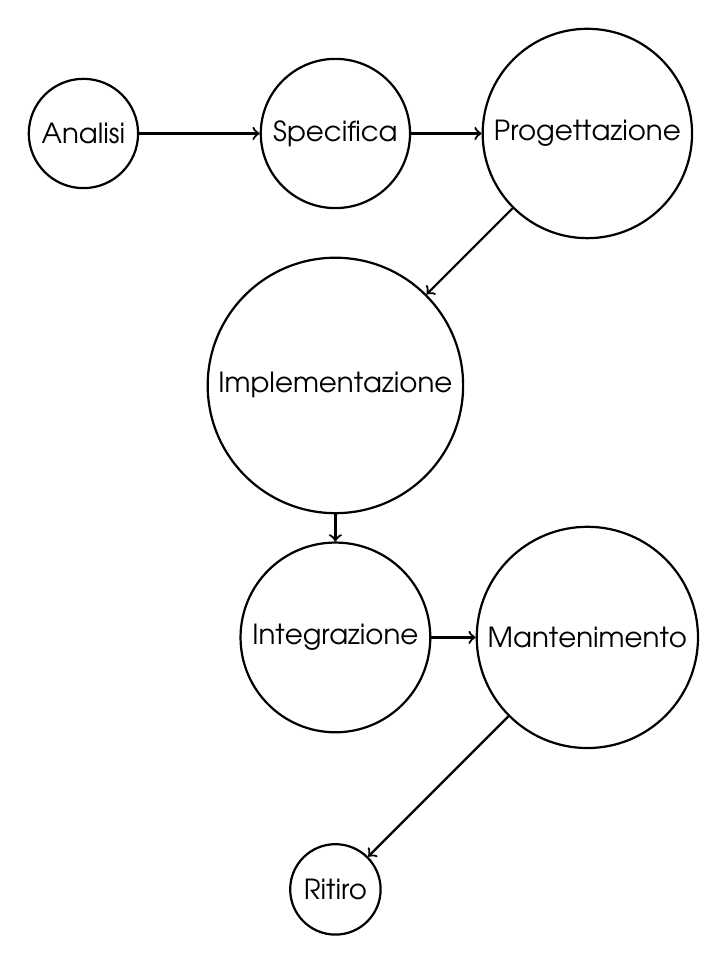
\begin{tikzpicture}[node distance={32mm}, thick, main/.style = {draw, circle}]
        \node[main] (1) {Analisi};
        \node[main] (2) [right of=1] {Specifica};
        \node[main] (3) [right of=2] {Progettazione}; 
        \node[main] (4) [below of=2] {Implementazione};
        \node[main] (5) [below of=4] {Integrazione}; 
        \node[main] (6) [right of=5] {Mantenimento};
        \node[main] (7) [below of=5] {Ritiro};
        \draw[->] (1) -- (2);
        \draw[->] (2) -- (3);
        \draw[->] (3) -- (4);
        \draw[->] (4) -- (5);
        \draw[->] (5) -- (6);
        \draw[->] (6) -- (7);
    \end{tikzpicture}
\end{center}
\subsection*{Specificità del Software}
    \begin{enumerate}
        \item \textbf{\textcolor{cyan}{Fault toulerance}}: capacità del software di essere tollerante ai guasti.
        \item \textbf{\textcolor{cyan}{Difetto latente}}: difetto nascosto che si trova difficilmente in fase di testing; e anche nel caso comparisse è quasi impossibile da ritrovare.
        \item \textbf{\textcolor{cyan}{Robustezza}}: capacità di funzionare anche con input non previsti e/o non testati.
        \item Il software non presenta \textcolor{cyan}{costi materiali} e nemmeno \textcolor{cyan}{costi marginali}, ovvero il costo di un'unità del prodotto.
        \item Infine il software non si consuma nel tempo, ma potrebbe diventare \textcolor{cyan}{obsoleto}.
    \end{enumerate}
\subsection*{La Manutenzione}
    \paragraph{Costi} 
    La fase di manutenzione è quella che richiede costi più alti. 
    Per evitare uno spreco durante questa fase è necessario studiare bene l'analisi dei requisiti, in quanto un errore in questa fase
    si propagherà in modo esponenziale, in termini di costi, nelle fasi successive.
    \break
    \break
    La manutenzione si divide in:
    \begin{itemize}
        \item \textbf{\textcolor{cyan}{Manutenzione Correttiva}}: rimuove gli errori, lasciando invariata la specifica.
        \item \textbf{\textcolor{cyan}{Manutenzione Migliorativa}}: consiste nel cambiare quella che è la specifica, e a sua volta può dividersi in:
            \begin{itemize}
                \item \textcolor{cyan}{Perfettiva}: modifiche per migliorare e/o introdurre nuove funzionalità.
                \item \textcolor{cyan}{Adattiva}: modifiche indotta da cambiamenti esterni, come leggi o modifiche all'hardware o al sistema operativo.
            \end{itemize}
    \end{itemize}
    \subsection*{Stakeholders}
        \begin{itemize}
            \item \textcolor{cyan}{Fornitore}: colui che sviluppa il software.
            \item \textcolor{cyan}{Committente}: chi lo richiede e paga.
            \item \textcolor{cyan}{Utente}: chi lo usa.
        \end{itemize}
        \section{Modelli di Ciclo di Vita}

\begin{definition}[Processo Software]
    Con processo software si indica il percorso da seguire per sviluppare un prodotto o più nello specifico un software.
    Fanno parte del processo sia gli strumenti e le tecniche per lo sviluppo che i professionisti coinvolti.
\end{definition}

\subsection{Modelli Sequenziali}

\subsubsection{Build-and-Fix}

Il prodotto è sviluppato senza alcuna fase di progettazione preliminare, lo sviluppatore scrive il software
e poi lo modifica ogni volta che non soffisfa il committente.

\paragraph{\textcolor{red}{Contro}}

Diventa improponibile per progetti grandi e la manutenzione diventa difficile senza documentazione nè specifica.

\subsubsection{Modello a Cascata}

Questo modello è stato il primo a distingure il processo software in più fasi, evidenziando l'importanza della progettazione e dell'analisi.

Viene chiamato anche modello \emph{\textcolor{cyan}{document driven}} dato che ogni fase produce un documento, e per passare alla successiva
occorre aver approvato il documento della fase precedente.

\paragraph{\textcolor{red}{Contro}} Troppo pesante da seguire, inoltre non si può tornare indietro, e mancando
l'interazione con il cliente, se non è soddisfatto, và tutto ripetuto dall'inizio.

\subsubsection{Modello a V}

\begin{center}
    \begin{figure}[h]
            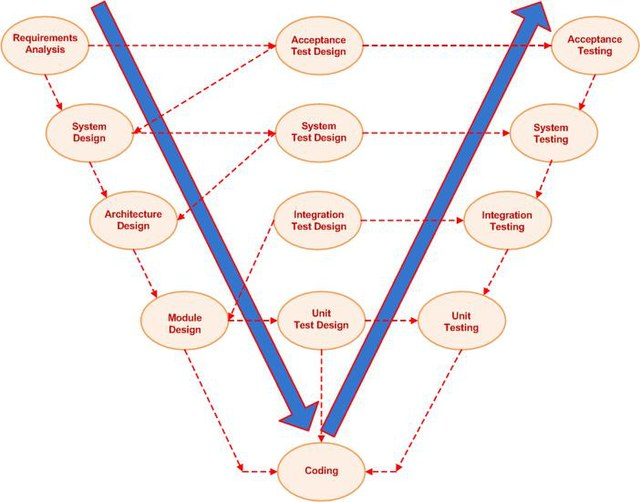
\includegraphics[scale=0.5]{img/V-model.JPG}
        \caption{Le frecce blu rappresentano il \emph{tempo}, mentre quelle tratteggiate le \emph{dipendenze}}
    \end{figure}
\end{center}

Questo modello evidenzia come sia possibile progettare i \textcolor{cyan}{test}
durante le fasi di sviluppo (quelle a sinistra, prima della fase di \emph{coding}). Mentre sulla destra
sono presenti i test veri e propri che devono verificare e convalidare l'attività in corrispondenza sulla sinistra.

\paragraph{\textcolor{ForestGreen}{Standard SQA}}
Questo modello è uno degli standard \emph{SQA} (Software Quality Assurance), usato
per descrivere le attività di test durante il processo di sviluppo.

\subsection{Modelli Iterativi}

\subsubsection{Rapid Prototyping}

L'obbiettivo è quello di costruire rapidamente un prototipo del software per permettere al committente di sperimentarlo.

Questo modello diventa utile quando i requisiti non sono chiari, quindi ogni prototipo aiuterà il cliente a descriverli meglio.

\begin{center}
    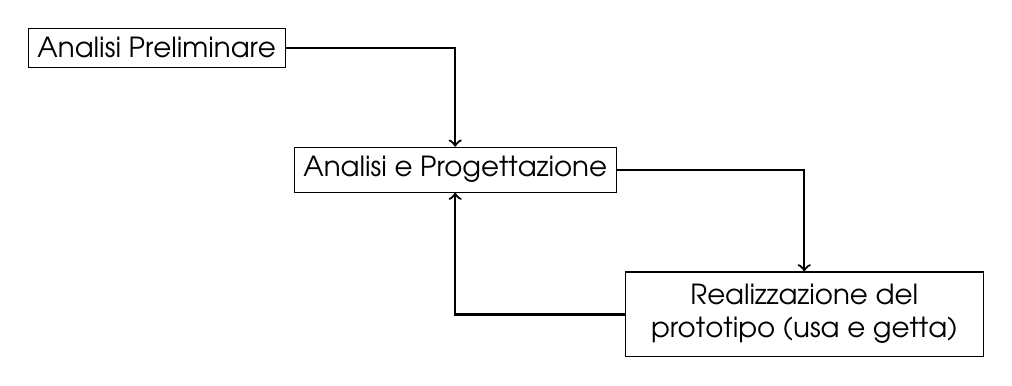
\begin{tikzpicture}[main/.style={rectangle, draw}]
        \node[main] (1) {Analisi Preliminare};
        \node[main] (2) [below right=1cm and 0.1cm of 1] {Analisi e Progettazione};
        \node[main] (3) [below right=1cm and 0.1cm of 2] {\begin{tabular}{c}Realizzazione del \\ prototipo (usa e getta)\end{tabular}};
        \draw[thick, ->] (1) -| (2);
        \draw[thick, ->] (2) -| (3);
        \draw[thick, ->] (3) -| (2);
    \end{tikzpicture}
\end{center}

\subsubsection{Modello Incrementale}

Il software viene costruito in modo iterativo, aggiungendo di volta in volta nuove funzionalità.

I requisiti e la progettazione vengono definiti inizialmente, per questo è possibile applicarlo solo in caso di requisiti stabili.

\paragraph{\textcolor{red}{Contro}}
Se non viene realizzata una buona progettazione, questo modello sfocia in un \emph{Build-and-Fix}.

\begin{center}
    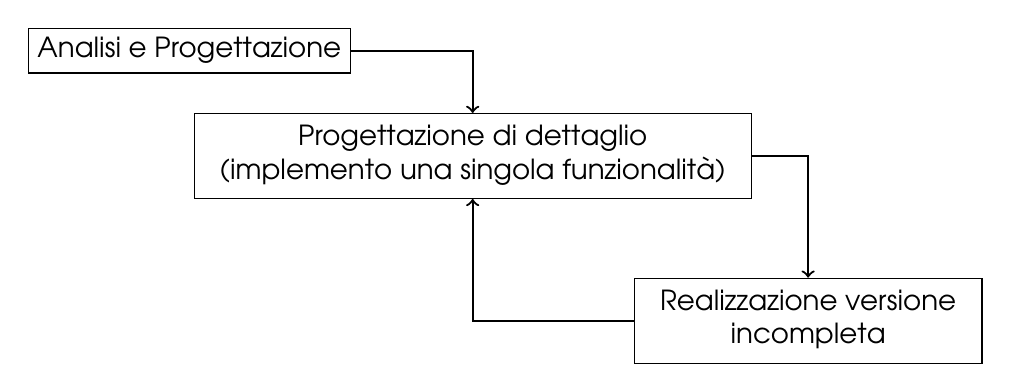
\begin{tikzpicture}[main/.style={rectangle, draw}]
        \node[main] (1) {Analisi e Progettazione};
        \node[main] (2) [below right=0.5cm and -2cm of 1] {\begin{tabular}{c} Progettazione di dettaglio \\ (implemento una singola funzionalità) \end{tabular}};
        \node[main] (3) [below right=1cm and -1.5cm of 2] {\begin{tabular}{c} Realizzazione versione \\ incompleta \end{tabular}};
        \draw[thick, ->] (1) -| (2);
        \draw[thick, ->] (2) -| (3);
        \draw[thick, ->] (3) -| (2);
    \end{tikzpicture}
\end{center}

\newpage

\subsubsection{Modello a Spirale}

In questo caso ogni iterazione è formata da 4 fasi che corrispondono ai quadranti del piano:
\begin{enumerate}
    \item \emph{Quadrante in alto a sinistra}: definizione degli obiettivi e dei vincoli.
    \item \emph{Quadrante in alto a destra}: analisi e risoluzione dei rischi.
    \item \emph{Quadrante in basso a destra}: sviluppo e verifica del prossimo livello.
    \item \emph{Quadrante in basso a sinistra}: pianificazione della fase successiva.
\end{enumerate}

Questo modello viene anche chiamato \emph{\textcolor{cyan}{risk driven}} in quanto è incentrato principalmente sull'analisi
dei rischi. Inoltre si ispira profondamente al metodo iterazivo \emph{\textcolor{cyan}{plan-do-check-act cycle}} \footnote{\url{https://it.wikipedia.org/wiki/Ciclo_di_Deming}}

\begin{figure}[h]
    \begin{center}
        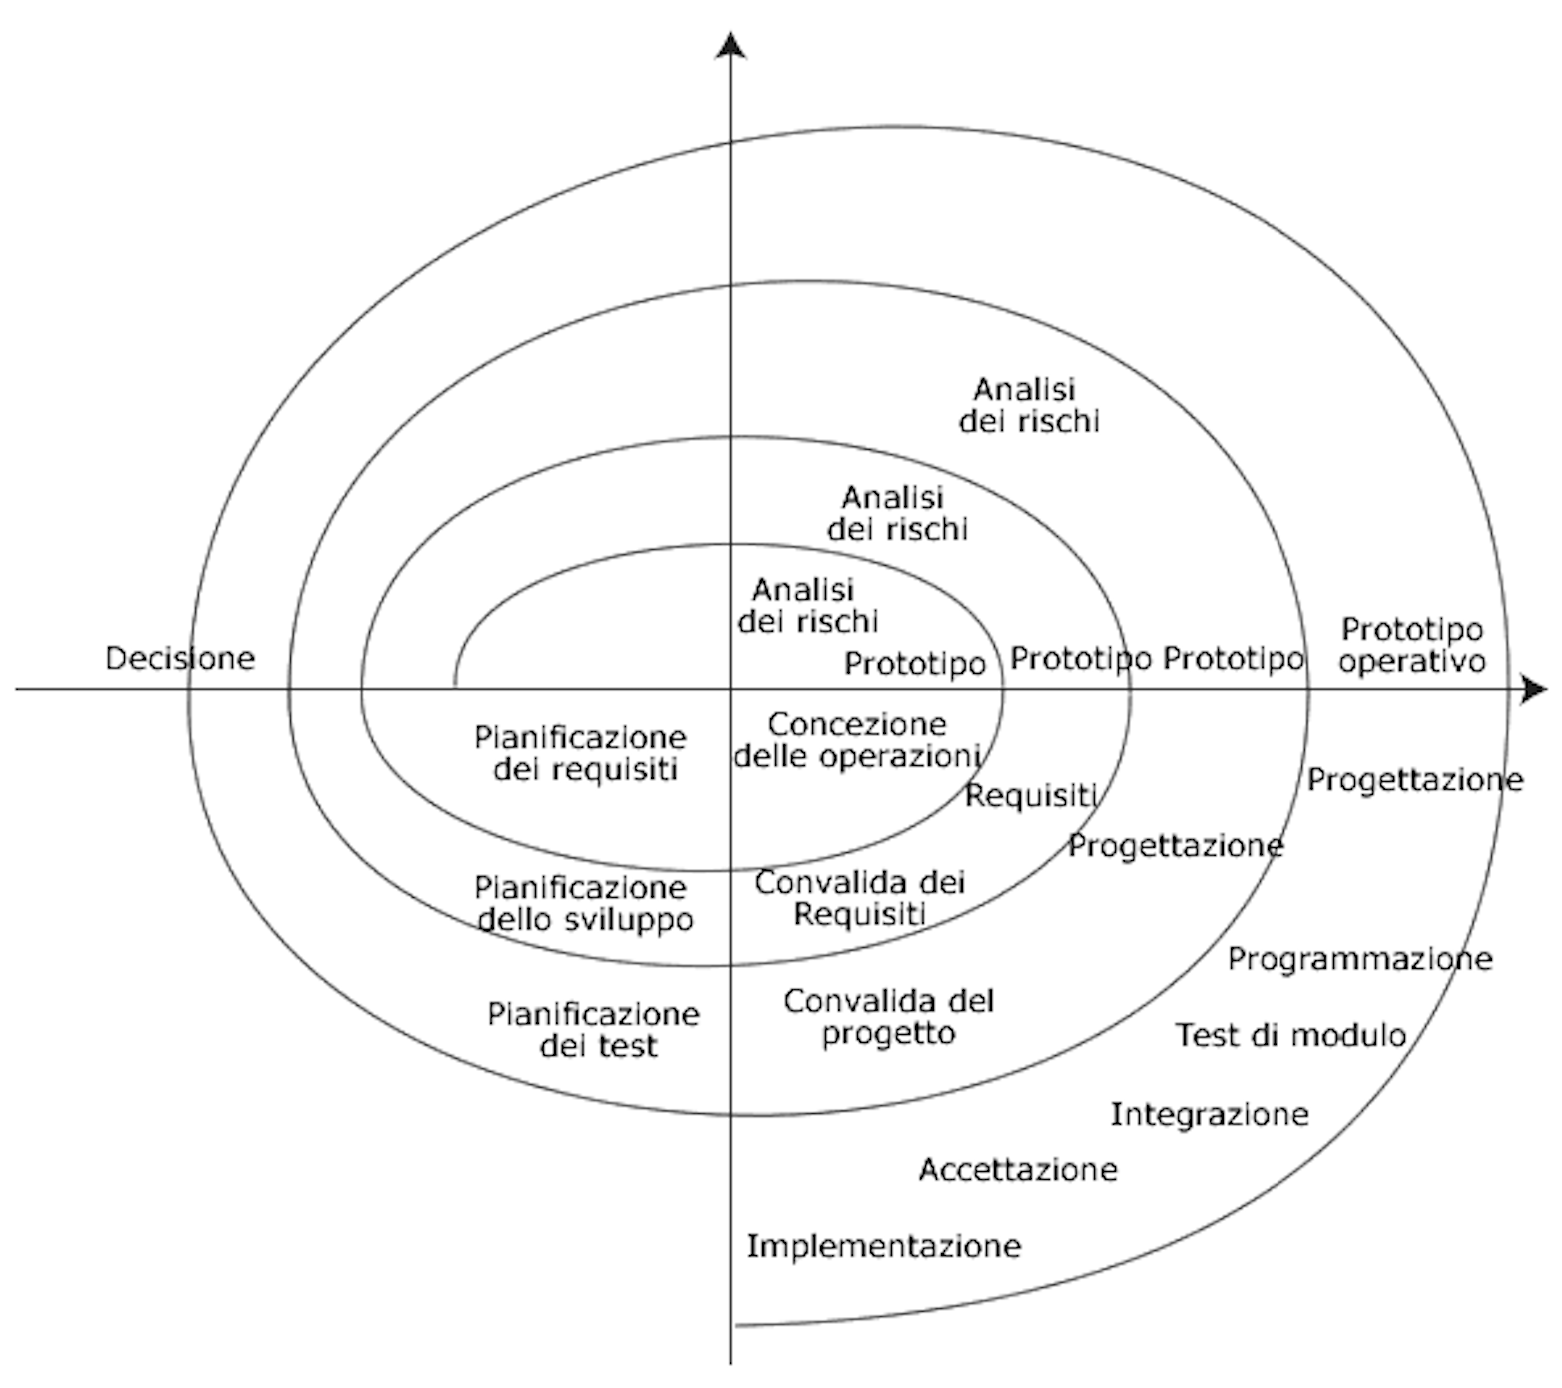
\includegraphics[scale=0.4]{img/modellospirale.png}
    \end{center}
\end{figure}

\subsection{Unified Process}

In questo modello vengono distinte quattro fasi chiamate \emph{\textcolor{cyan}{Inception}}, \emph{\textcolor{cyan}{Elaboration}}, \emph{\textcolor{cyan}{Construction}}
e \emph{\textcolor{cyan}{Transition}}. Ogni fase può presentare un numero variabile di iterazioni anche in base alla dimensione
del progetto.

Questo modello viene definito \textcolor{cyan}{iterativo incrementale}, \emph{incrementale} perchè
alla fine di ogni iterazione si ottiene un rilascio del sistema con funzionalità in più o migliorate
rispetto al rilascio precedente.

Inoltre viene data molta importanza all'architettura del sistema, infatti già dalle prime fasi ci si
concentra soprattutto sull'architettura anche se a livello molto superficiale, lasciando i dettagli alle fasi successive. In questo
modo è molto facile avere una visione generale del sistema che sarà facilmente modellabile sulla variazione dei requisiti. Per
questo, piuttosto che dai requisiti, ci si fà guidare principalmente dai \emph{casi d'uso} e dall'\emph{analisi dei rischi}.

\begin{figure}[h]
    \begin{center}
        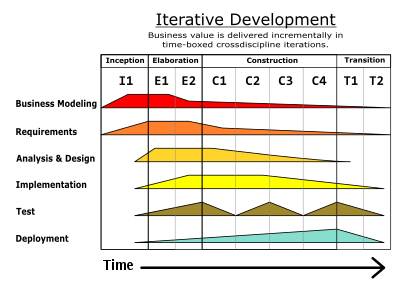
\includegraphics[scale=0.8]{img/unified_process.png}
    \end{center}
\end{figure}

\subsection{Processi Agili}

\begin{definition}[Metodo Agile]
    Con \textcolor{cyan}{metodo agile} si intende un metodo per lo sviluppo del software
    che si basa principalmente sul coinvolgimento del committente.
    Questa metodologia si riferisce ai principi del \emph{\textcolor{cyan}{Manifesto di Snowbird}} del 2001.
\end{definition}

I concetti chiave di questi processi sono:

\begin{itemize}
    \item \textcolor{cyan}{Continuous Integration}: rendere il più automatico possibile la consegna e l'integrazione dei singoli moduli.
    \item \textcolor{cyan}{Continuous Delivery}: rilascio frequente e supportato delle nuovi versioni del software.
    \item \textcolor{cyan}{DevOps}: \emph{Development} e \emph{Operations}, ovvero maggiore collaborazione tra sviluppatori e responsabili della
        manutenzione, della sicurezza e dell'infrastruttura dell'azienda.
\end{itemize}

\subsubsection{Il Manifesto di Snowbird}

Il \emph{Manifesto di Snowbird} si fonda su quattro punti fondamentali:

\begin{enumerate}
    \item \textcolor{cyan}{Comunicazione}: la comunicazione fra tutti gli attori del progetto è centrale, soprattutto le interazioni e
        la collaborazione con i clienti.
    \item \textcolor{cyan}{Semplicità}: si mantiene il codice sorgente il più semplice possibile, ma comunque avanzato tecnicamente,
        in questo modo si riduce la documentazione al minimo indispensabile.
    \item \textcolor{cyan}{Feedback}: sin dal primo giorno di sviluppo il codice viene testato, in modo da poter rilasciare versioni ad intervalli molto frequenti.
    \item \textcolor{cyan}{Coraggio}: dare in uso il sistema il prima possibile ed implementare i cambiamenti richiesti man mano.
\end{enumerate}

Di seguito sono riportati due modelli che si basano sui \emph{processi agili}.

\subsubsection{eXtreme Programming}

Si basa su un insieme di consuetudini:

\begin{itemize}
    \item \emph{Pianificazione flessibile}: è basata su un insieme di scenari proposti dagli utenti e i programmatori vengono coinvolti direttamente.
    \item \emph{Rilasci frequenti}: più o meno ogni 2-4 settimane, e alla fine si ricomincia con una nuova pianificazione.
    \item \emph{Progetti semplici}: comprensibili a tutti.
    \item \emph{Testing}: test basati sui singoli scenari e con supporto automatico.
    \item \emph{Test Driven Development}: i casi di test vengono definiti prima della scrittura del codice.
    \item \emph{Cliente sempre a disposizione}
    \item \emph{Programmazione a coppie}: viene usato un solo terminale, una persona svolge il ruolo di \emph{\textcolor{cyan}{driver}}
        che scrive il codice, mentre un'altra fà il \emph{\textcolor{cyan}{navigatore}}, ovvero controlla il lavoro del \emph{driver} attivamente.
    \item \emph{No al lavoro straordinario}
    \item \emph{Collettivizzazione del codice}: accesso libero e continua integrazione.
    \item \emph{Code Refactoring}: modificare il codice senza cambiare il suo comportamento e commentarlo il più possibile.
    \item \emph{Daily Stand Up Meeting}
\end{itemize}

\subsubsection{SCRUM}

\begin{definition}[SCRUM]
    Con \emph{\textcolor{cyan}{SCRUM}} si intende un processo \emph{iterativo} ed \emph{incrementale}, dove alla fine
    di ogni iterazione vengono rilasciate un insieme di funzionalità potenzialmente rilasciabili.
\end{definition}

Il processo è diviso in tre fasi:

\begin{enumerate}
    \item \textbf{\textcolor{cyan}{Pre-game phase}}: 
        \begin{enumerate}
            \item \textcolor{cyan}{Planning sub-phase}: viene creata una \emph{\textcolor{cyan}{Product Backlog List}}
                che contiene tutti i requisiti conosciuti.
            \item \textcolor{cyan}{Architecture sub-phase}: viene già pianificato il design di alto livello e l'architettura del sistema.
        \end{enumerate}
    \item \textbf{\textcolor{cyan}{Development phase}}: in questa fase il sistema viene sviluppato attraverso una serie di \emph{\textcolor{cyan}{Sprint}},
        ovvero cicli iterativi nei quali vengono sviluppate o migliorate una serie di funzionalità, e ogni sprint può durare circa 1-4 settimane. Lo \emph{Sprint} ovviamente
        include le classiche fasi di sviluppo del software.
    \item \textbf{\textcolor{cyan}{Post-game phase}}: il prodotto viene preparato per il rilascio, ovvero si prepara l'\emph{integrazione},
        i \emph{test}, la \emph{documentazione} per l'utente e la preparazione del materiale di \emph{marketing}.
\end{enumerate}

I ruoli principali durante l'esecuzione di un processo \emph{SCRUM} sono tre:

\begin{itemize}
    \item \textbf{\textcolor{cyan}{Product Owner}}: ci si riferisce a quella persona responsabile di accettare o rifiutare i risultati di un lavoro e di poter terminare uno \emph{Sprint}, inoltre
        fà da raccordo fra tutti soggetti interessati nel progetto.
    \item \textbf{\textcolor{cyan}{Membri del Team}}: i membri decidono cosa fare in ogni \emph{Sprint}, ogni team è indipendente e i membri non fanno capo ad alcun project manager.
        Ogni membro ha diverse specializzazioni (\emph{cross-functional}), in modo tale da non avere persone con troppo carico di lavoro e ognuno si occupa di un singolo lavoro alla volta.
    \item \textbf{\textcolor{cyan}{Scrum Master}}: non ha alcuna autorità sul team, ma si occupa di supportarlo e motivarlo, garantendo anche le condizioni ambientali per lavorare al meglio.
\end{itemize}

\paragraph{Kanban Board} Questa lavagna permette di gestire al meglio il flusso del lavoro. Come mostrato in figura è presente
un \emph{\textcolor{cyan}{Work In Progress Limit}} che definisce un limite alla quantità di post-it che possono essere presenti in
ogni colonna. Questo limite permette di completare più velocemente i singoli lavori, in modo tale di dare qualcosa al cliente il prima possibile e di
individuare facilmente i \textcolor{cyan}{colli di bottiglia} che possono rallentare gli altri lavori.
Inoltre permette di ridurre il \emph{\textcolor{cyan}{task switching}}, ovvero il lavoro su più task contemporaneamente.

\begin{figure}[h]
    \begin{center}
        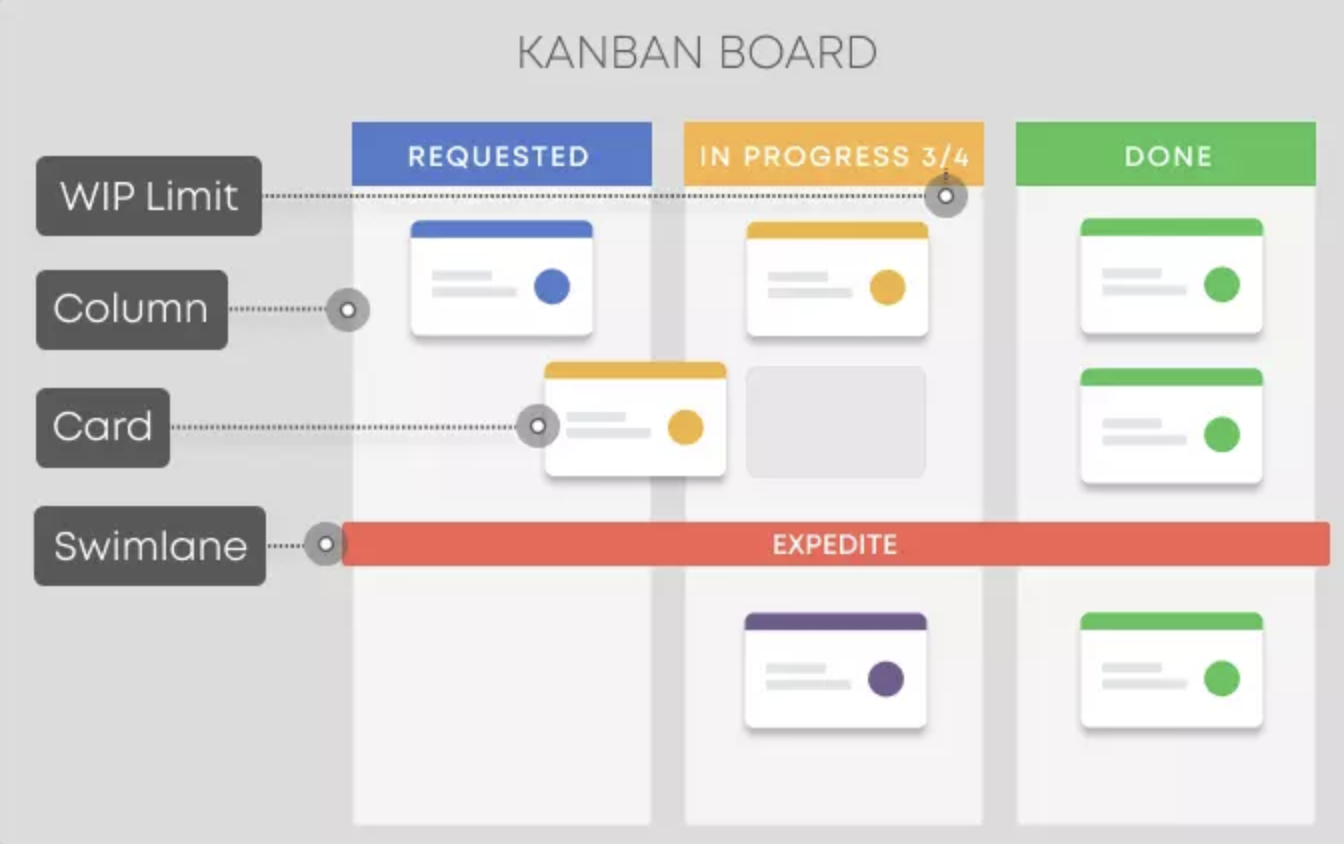
\includegraphics[scale=0.5]{img/kanboard.png}
    \end{center}
\end{figure}

Gli eventi che fanno parte di uno \emph{Sprint} sono i seguenti:
\begin{enumerate}
    \item \textcolor{cyan}{Sprint planning}: il \emph{product owner} gestisce l'evento di pianificazione dello \emph{Sprint}.
    \item \textcolor{cyan}{Daily meeting}: i membri del team e gli SCRUM master si ritrovano davanti la \emph{kanban} e discutono delle
        difficultà che hanno riscontrato.
    \item \textcolor{cyan}{Review}: alla fine di di una modifica concreta al software, questo viene ispezionato in collaborazione con gli utenti per ottenere un feedback
        e per discutere su cambiamenti o nuove idee.
    \item \textcolor{cyan}{Retrospettiva}: questa fase permette di riflettere, studiare e adattarsi per lo \emph{Sprint} successivo.
\end{enumerate}
        \section{Analisi dei Requisiti}

\begin{definition}[Analisi dei Requisiti]
    Si intende il processo di studio e analisi delle esigenze del committente e dell'utente per
    giungere alla produzione di un documento che definisce il \emph{dominio} del problema e i \emph{requisiti} del software.
    In alcuni casi si definiscono anche i \emph{casi di test} e il \emph{manuale utente}.
\end{definition}

Prima di passare alla fase vera e propria di \emph{analisi dei requisiti}
occorre seguire una fase preliminare per stabilire la realizzabilità
del progetto software.

\subsection{Studio di Fattibilità}

Si basa principalmente sulla descrizione del software e delle necessità
dell'utente. In seguito vengono svolte due analisi:

\begin{itemize}
    \item \textcolor{cyan}{Analisi di Mercato}: si fà un confronto con il mercato attuale e si stimano i costi di
        produzione e quanto l'investimento può essere remunerativo.
    \item \textcolor{cyan}{Analisi Tecnica}: si studiano tutti gli strumenti per la realizzazione del progetto,
        come i software, le architetture, gli hardware e gli algoritmi. Inoltre si studia come deve essere fatta la prototipazione
        del software e la futura ricerca. 
\end{itemize}

\subsection{Dominio}

Il \textbf{\textcolor{cyan}{dominio}} è il contesto in cui il software opera. Per definirlo occorre costruire
un \textcolor{cyan}{glossario}, ovvero una collezione di definizioni di termini rilevanti in quel dominio specifico e
che può essere riusato in progetti successivi nello stesso dominio. Inoltre occorre definire un \textcolor{cyan}{modello statico},
quindi come interagiscono fra loro gli elementi del dominio staticamente, e un \textcolor{cyan}{modello dinamico}, ovvero come si comporta il dominio
in base all'avvenire di un determinato evento che può coinvolgere gli utenti. Questi due modelli possono essere descritti sia 
tramite l'uso del linguaggio UML \footnote{\url{https://it.wikipedia.org/wiki/Unified_Modeling_Language}}, sia usando la semplice descrizione testuale.

\subsection{Requisiti}

\begin{definition}[Requisito]
    Il requisito è una proprietà che deve essere garantita dal sistema per soddisfare
    una qualsiasi necessità dell'utente.
\end{definition}

I requisiti possono dividersi in due categorie:
\begin{itemize}
    \item \textbf{\textcolor{cyan}{Requisiti funzionali}}: quelli che descrivono le funzionalità e il comportamento del software.
    \item \textbf{\textcolor{cyan}{Requisiti non funzionali}}: descrivono le proprietà del software o del processo di sviluppo. Ad esemprio le caratteristiche di
        efficienza e affidabilità, l'interfaccia, il linguaggio di programmazione e l'ambiente di sviluppo scelti, i vincoli legislativi e i requisiti hardware o di rete.
\end{itemize}

I requisiti possono essere descritti mediante l'uso di diversi linguaggi, formali o meno. In questo caso si vede
la descrizione dei requisiti mediante la produzione di un documento scritto in linguaggio naturale.

\subsection{Documento dei Requisiti}

Questo documento è un contratto tra lo sviluppatore e il committente, che elenca i requisti e i vincoli che il software deve soddisfare, e specifica
anche una \emph{deadline} per la consegna del progetto.

\subsection{Fasi dell'Analisi dei Requisiti}

L'\emph{analisi dei requisiti} viene svolta in cinque passi:
\begin{enumerate}
    \item \textbf{\textcolor{cyan}{Acquisizione}}
    \item \textbf{\textcolor{cyan}{Elaborazione}}
    \item \textbf{\textcolor{cyan}{Convalida}}
    \item \textbf{\textcolor{cyan}{Negozazione}}
    \item \textbf{\textcolor{cyan}{Gestione}}
\end{enumerate}

\subsubsection{Acquisizione}

Il team di analisti incontra i membri dell'organizzazione del committente e si procede con
la raccolta dei requisiti che può avvenire tramite: semplici interviste, questionari, costruzione di
prototipi (anche su carta), studio di documenti o l'osservazione di possibili utenti mentre lavorano.

\subsubsection{Elaborazione}

Viene scritta la prima bozza del \emph{documento dei requisti}, dove quest'ultimi vengono trattati in modo
più approfondito. La struttura del documento deve essere la seguente:

\begin{center}
    \begin{tabular}{||c||}
        \hline
        \emph{Introduzione} \\
        \hline
        \emph{Glossario} \\
        \hline
        \emph{Definizione dei Requisiti Funzionali} \\
        \hline
        \emph{Definizione dei Requisiti Non Funzionali} \\
        \hline
        \emph{Architettura}: la strutturazione del software in sottosistemi. \\
        \hline
        \emph{Specifica dettagliata dei Requisiti Funzionali} \\
        \hline
        \emph{Modelli astratti}: descrivere il sistema in base \\ a ciascun punto di vista. \\
        \hline
        \emph{Evoluzione del sistema}: successivi cambiamenti. \\
        \hline
        \emph{Appendici}: descrizione della piattaforma hardware, database, \\ manuale utente e i piani di test. \\
        \hline
        \emph{Indici}: costruire un lemmario, quindi una lista di termini \\ che puntano ai requisiti che li usano. \\
        \hline
    \end{tabular}
\end{center}

\paragraph{Nota Bene} Nella descrizione dei requisiti occorre sempre usare la forma assertiva.
Esempio:
\begin{center}
    \emph{Il $<$sistema$>$ deve $<$funzionalità$>$/$<$proprietà$>$}
\end{center}

\subsubsection{Convalida}

Nella fase di convalida occorre revisionare il documento per far sì che vengano
evitati i seguenti difetti:

\begin{itemize}
    \item \textcolor{cyan}{Omissioni}: requisiti mancanti.
    \item \textcolor{cyan}{Inconsistenze}: contraddizione tra i requisiti o tra un requisito e il contesto.
    \item \textcolor{cyan}{Ambiguità}: vaghezze o requisiti che possono avere più significati. Le ambiguità all'interno del linguaggio naturale
        possono essere portate da \textcolor{MidnightBlue}{quantificatori}, \textcolor{MidnightBlue}{disgiunzioni}
        oppure possono presentarsi ambiguità di \textcolor{MidnightBlue}{coordinazione} (nel caso si usano sia la \emph{o} che la \emph{e} nella stessa frase) oppure 
        \textcolor{MidnightBlue}{referenziale} nell'uso non chiaro di pronomi.
        Inoltre occorre sempre evitare \textcolor{MidnightBlue}{verbi deboli}, \textcolor{MidnightBlue}{forme passive}, ovvero verbi senza un soggetto esplicito ed anche \textcolor{MidnightBlue}{negazione}
        e \textcolor{MidnightBlue}{doppie negazioni}.
    \item \textcolor{cyan}{Sinonimi} e \textcolor{cyan}{Omonimi}: termini diversi con lo stesso significato e termini uguali con significato diverso.
    \item \textcolor{cyan}{Presenza di dettagli tecnici}
    \item \textcolor{cyan}{Ridondanza}: può esserci, ma solo tra sezioni diverse del documento.
\end{itemize}

Le principali tecniche di convalida dei requisiti sono:
\begin{itemize}
    \item \textcolor{cyan}{Deskcheck}
        \begin{itemize}
            \item \textcolor{cyan}{Walkthrough}: ovvero il documento viene analizzato per intero sequenzialmente.
            \item \textcolor{cyan}{Ispezione}: la lettura del documento è strutturata, utilizzando per esempio la tecnica del
                lemmario.
        \end{itemize}
    \item Uso di \textcolor{cyan}{strumenti di analisi} del linguaggio naturale.
    \item Uso di \textcolor{cyan}{prototipi}.
\end{itemize}

Una volta trovati i difetti, è importante ricordarsi che vanno sempre risolti con
il committente.

\subsubsection{Negoziazione}

In questa fase vengono assegnate delle priorità ai requisiti in base alle
\textcolor{cyan}{esigenze del committente} e ai \textcolor{cyan}{costi} e \textcolor{cyan}{tempi} di
produzione.

Questa fase è importante per decidere se alcuni requisiti possono essere \textcolor{cyan}{cancellati} oppure
\textcolor{cyan}{sviluppati} successivamente.

\paragraph{MoSCoW} Questa è una tecnica per dare priorità ai requisiti, i quali vengono divisi in quattro classi:
\begin{itemize}
    \item \textcolor{cyan}{Must have}: requisiti irrinunciabili per il cliente.
    \item \textcolor{cyan}{Should have}: non necessari ma utili.
    \item \textcolor{cyan}{Could have}: non molto utili, da realizzare solo se c'è tempo.
    \item \textcolor{cyan}{Want to have}: da sviluppare in successive versioni.
\end{itemize}

\subsubsection{Gestione}

Questa fase si occupa di tre aspetti principali:
\begin{itemize}
    \item \textcolor{cyan}{Identificazione}: ad ogni requisito viene assegnato un identificatore univoco.
    \item \textcolor{cyan}{Attributi}: ad ogni requisito vengono assegnati attributi relativi allo \textcolor{MidnightBlue}{stato},
        \textcolor{MidnightBlue}{priorità}, \textcolor{MidnightBlue}{sforzo} in termini di giorni e/o personale da impiegare, \textcolor{MidnightBlue}{rischio},
        e la \textcolor{MidnightBlue}{versione destinazione} per quanto riguarda lo sviluppo incrementale. 
    \item \textcolor{cyan}{Tracciabilità}: ovvero la capacità di descrivere e seguire la vita di un requisito. Viene costruita una mappa tra i requisiti
        e le \textcolor{MidnightBlue}{componenti del sistema}, il \textcolor{MidnightBlue}{codice} ed i \textcolor{MidnightBlue}{test}.
\end{itemize}

\paragraph{Contratto} Il \emph{documento dei requisiti} precede la stipula del contratto.

\subsection{Casi d'uso}

I \textbf{\textcolor{cyan}{casi d'uso}} sono un altro modo per acquisire i requisiti, valutando le interazioni degli utenti col sistema
e indicando al committente i risultati attesi. I casi d'uso oltre ad includere la sequenza corretta di eventi attesi devono anche presentare i comportamenti inattesi,
ovvero le \textcolor{cyan}{eccezioni}.

\subsection{User Stories}

Sono un'altra tecnica di raccolta dei requisiti utilizzata principalmente nei \emph{\textcolor{cyan}{processi agile}} e consiste
nell'utilizzo di \emph{\textcolor{cyan}{user story cards}} per scrivere i requisiti, che in linea generale hanno questa forma:
\begin{center}
    \emph{Nel mio ruolo di $<$ruolo utente$>$, ho bisogno che il sistema $<$obiettivo$>$, al fine di $<$beneficio$>$}
\end{center}

\paragraph{\textcolor{red}{Contro}} Il problema principale delle \emph{user stories} è la \textcolor{cyan}{scalabilità}, 
ovvero sono difficili da trasporre su grandi progetti e problematiche se il team è distribuito geograficamente. Inoltre, essendo
informali e brevi non sono adatte per raggiungere degli accordi legali e raramente includono i \emph{requisiti non funzionali}.
        \newpage

\section{Linguaggio UML e Casi d'Uso}

\begin{definition}[Modello]
    Un \emph{modello} è un'astrazione del dominio, usato per specificarne la natura e il comportamento.
\end{definition}

I modelli possono classificarsi in:
\begin{itemize}
    \item \textbf{\textcolor{cyan}{Modelli Statici}}: vengono rappresentate le \emph{entità} e le \emph{relazioni} fra esse per permettere di descrivere al meglio
        il dominio, le componenti architetturali e le classi da realizzare.
    \item \textbf{\textcolor{cyan}{Modelli Dinamici}}: vengono modellati i comportamenti delle entità descritte nel \emph{modello statico}.
\end{itemize}

Un modello può essere:
\begin{itemize}
    \item Una \textcolor{cyan}{bozza} o \textcolor{cyan}{sketch}, quindi un modello molto incompleto,
        usato principalmente per descrizioni iniziali.
    \item Un progetto dettagliato chiamato \textcolor{cyan}{blueprint},
        che permette ai programmatori di realizzare direttamente il software senza prendere decisioni di
        progettazione.
    \item Un \textcolor{cyan}{eseguibile}, talmente preciso e completo da poter generare il codice
        in automatico partendo solo dal modello.
\end{itemize}

\subsection{UML}

\begin{definition}[UML]
    L'\emph{Unified Modeling Language} è un linguaggio di modellazione unificato che ha il compito
    di supportare la descrizione e il progetto di software, nello specifico di applicazioni \emph{object oriented}, ma permette
    anche di descrivere i modelli da più punti di vista in modo molto comprensibile sia dai clienti che dagli utenti.
\end{definition}

\subsection{Diagramma dei Casi d'Uso}
Permette di descrivere i \emph{\textcolor{cyan}{requisiti funzionali}} del sistema, catturando nello specifico
le funzionalità viste dall'esterno (lato utente).

\begin{definition}[Attore]
    Un \textbf{\textcolor{cyan}{attore}} è un'entità esterna al sistema, che interagisce con esso.
    Gli attori possono essere classificati in:
    \begin{itemize}
        \item Un \textcolor{cyan}{utente umano} che possiede un determinato ruolo.
        \item Un altro \textcolor{cyan}{sistema}.
        \item Il \textcolor{cyan}{tempo}.
    \end{itemize}
    All'interno del diagramma gli attori sono delle classi e sono indicati con un nome in maiuscolo.
\end{definition}

\begin{definition}[Caso d'Uso]
    Un \textbf{\textcolor{cyan}{caso d'uso}} è una funzionalità o un servizio offerto dal sistema a uno o più attori, e viene
    espresso tramite un insieme di \emph{scenari}.

    All'interno del diagramma, anche i casi d'uso sono scritti in maiuscolo, e per descriverli vengono usati dei \emph{verbi} che ne indicano il compito.
\end{definition}

Il \emph{\textcolor{cyan}{diagramma dei casi d'uso}} oltre ad essere composto da
\emph{attori} e da \emph{casi d'uso}, presenta anche:
\begin{itemize}
    \item \textcolor{cyan}{Relazioni}: tra gli attori e i casi d'uso che rappresentano un'interazione.
    \item Il \textcolor{cyan}{confine del sistema}: un rettangolo disegnato intorno ai casi d'uso per indicare il confine del sistema.
\end{itemize}

È importante specificare che un caso d'uso è sempre iniziato da un solo attore, chiamato \textcolor{cyan}{attore principale}. Inoltre, possono
essere presenti casi d'uso non collegati ad alcun attore.

\begin{figure}[h]
    \centering
\end{figure}

\subsection{Narrativa dei Casi d'Uso}
Per poter descrivere il \emph{modello dinamico}, viene redatto un documento che permette di
rappresentare gli scenari di ogni caso d'uso dal punto di vista di ogni attore coinvolto.

\begin{definition}[Precondizioni e postcondizioni]
    Le \textbf{\textcolor{cyan}{precondizioni}} e le \textbf{\textcolor{cyan}{postcondizioni}} sono
    dei predicati che devono sempre essere veri in uno stato: per le \emph{precondizioni} prima di iniziare il caso d'uso,
    per le \emph{postcondizioni} alla fine.
\end{definition}

La descrizione di un caso d'uso segue questa struttura:

\begin{center}
    \begin{tabular}{||c||}
        \hline
        \emph{Nome} \\
        \hline
        \emph{Breve descrizione} \\
        \hline
        \emph{Attore primario} \\
        \hline
        \emph{Attori secondari} \\
        \hline
        \emph{Precondizioni} \\
        \hline
        \emph{Sequenza degli eventi principale} \\
        \hline
        \emph{Postcondizioni} \\
        \hline
        \emph{Sequenze alternative degli eventi} \\
        \hline
    \end{tabular}
\end{center}

\begin{definition}[Scenario]
    Uno \textbf{\textcolor{cyan}{scenario}} è un'istanza di un caso d'uso, ovvero una sequenza 
    di interazioni tra il sistema e gli attori che produce un risultato osservabile.

    Gli scenari descritti dalla \emph{sequenza degli eventi principale} sono quelli che portano
    alle \emph{postcondizioni}.
\end{definition}

La \emph{\textcolor{cyan}{Sequenza degli eventi principale}} elenca i passi che compongono il caso d'uso ed ogni passo presenta la
seguente sintassi:
\begin{center}
    \verb|<|\emph{numero}\verb|>|. \verb|<|\emph{soggetto}\verb|><|\emph{azione}\verb|><|\emph{complementi}\verb|>|
\end{center}
Il primo passo, inoltre, è sempre compiuto dall'\emph{attore principale}.
All'interno della sequenza possono anche presenti \emph{condizioni} e \emph{cicli}, scritti in pseudocodice.

%manca immagine, approfondimento hoare e liskov.

\subsubsection{Inclusione}

L'\emph{\textcolor{cyan}{inclusione}} permette di creare una relazione di dipendenza tra casi d'uso.

È importante non usare la relazione di inclusione per fare decomposizione di un caso d'uso.

\subsubsection{Estensione}

L'\emph{\textcolor{cyan}{estensione}}, a differenza dell'\emph{inclusione}, non è una dipendenza, ma
permette a un caso d'uso di incorporarne opzionalmente un altro.
        \subsection{Classi e Oggetti}

\begin{definition}[Oggetto]
    Un \textbf{\textcolor{cyan}{oggetto}} è un entità caratterizzata da un'\emph{\textcolor{cyan}{identità}},
    uno \emph{\textcolor{cyan}{stato}}, ovvero i valori degli \emph{attributi} dell'oggetto, e da un \emph{\textcolor{cyan}{comportamento}},
    quindi le operazioni che lo definiscono.
\end{definition}

\begin{definition}[Classe]
    Una \textbf{\textcolor{cyan}{classe}} è un insieme di \emph{oggetti} con caratteristiche simili,
    quindi che hanno lo stesso tipo.

    Una classe permette di catturare gli elementi del dominio del sistema.
\end{definition}

\subsubsection{Diagramma delle Classi}

Descrive le \textcolor{cyan}{proprietà} e le \textcolor{cyan}{operazioni} di un classe, il \textcolor{cyan}{tipo degli oggetti}, e le \textcolor{cyan}{relazioni \emph{statiche}} fra essi.

\begin{wrapfigure}{l}{0.\textwidth}
    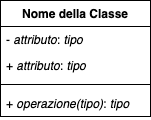
\includegraphics[scale=0.7]{img/diagrammaclassi.png}
\end{wrapfigure}

Una classe viene rappresentata in questo modo, con il nome sempre in maiuscolo, la sezione che riguarda gli attributi
e quella che riguarda le operazioni. Il simbolo \textbf{\textcolor{MidnightBlue}{$+$}} indica un attributo/operazione privata, mentre il \textbf{\textcolor{MidnightBlue}{$-$}} ne indica uno
pubblico. Esistono anche altri due simboli per la \emph{\textcolor{cyan}{visibilità}}: il \textbf{\textcolor{MidnightBlue}{$\#$}}, che indica
che l'attributo o l'operazione è accessibile anche alle classi discendenti nella \textcolor{cyan}{gerarchia}, mentre la
\textbf{\textcolor{MidnightBlue}{$\sim$}} che indica l'accessibilità solo alle classi nello stesso \emph{package}.
Inoltre, per specificare che un attributo o un'operazione sono \emph{\textcolor{cyan}{statici}}, si sottolineano.

Nonostante ciò, quando si usa il diagramma delle classi per descrivere il dominio, sia le operazioni che la visibilità
e i dettagli implementativi degli attributi si omettono.

\paragraph{Attributi} La sintassi degli attributi è la seguente:
\begin{center}
    \verb|Visibilità Nome: Tipo[Molteplicità] = ValoreDefault {Proprietà}| 
\end{center}
La \textcolor{cyan}{\emph{molteplicità}} indica gli array di valori, quando è uguale a $1$ può essere omessa.
Invece, le \textcolor{cyan}{\emph{proprietà}} possono essere sui valori dell'attributo, oppure nel caso la molteplicità è maggiore di $1$ si può
usare \verb|{ordered}| per indicare che nell'array l'ordine degli elementi conta, e \verb|{unique}| per dire che gli elementi
dell'array non devono avere ripetizioni.

\paragraph{Operazioni} La sintassi delle operazioni è la seguente:
\begin{center}
    \verb|Visibilità Nome: (ListaParametri) : TipoRitorno| 
\end{center}
Con \verb|ListaParametri| definita dalla seguente grammatica:
\[
    ListaParametri::=\;\varnothing\;|\;DichiarazioneParametro,\;ListaParametri
\]
\[
    DichiarazioneParametro::=\;Nome:\;Tipo\;=\;ValoreDefault
\]

\paragraph{Enumerazioni} Sono usate per specificare una lista prefissata di valori che un \emph{\textcolor{cyan}{attributo}} può assumere.
In UML sono etichettate con lo stereotipo \verb|<<enumeration>>|.
\begin{figure}[h]
    \centering
    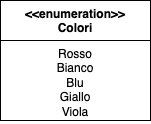
\includegraphics[scale=0.7]{img/enumeration.png}
    \caption{\begin{tabular}{c}Esempio di enumerazione con l'attributo \emph{colore}.\end{tabular}}
\end{figure}

\subsubsection{Relazioni}

\begin{definition}[Relazione]
    Una \textbf{\textcolor{cyan}{relazione}} rappresenta un legame tra due o più oggetti.

    In UML viene rappresentata da una linea retta con sopra scritte il \textcolor{cyan}{nome dell'associazione}, il \textcolor{cyan}{ruolo} di ogni classe, ed
    eventualmente una freccia che sta ad indicare il verso di lettura dell'associazione.

    In generale si usa specificare o solo il \emph{nome dell'associazione} o solo i \emph{ruoli}.
\end{definition}

\begin{figure}[h]
    \centering
    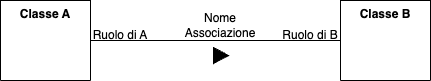
\includegraphics[scale=0.7]{img/relazione.png}
\end{figure}

\newpage
\paragraph{\textcolor{cyan}{Molteplicità}} La \emph{molteplicità} indica il numero di oggetti
coinvolti in un'associazione in un dato istante. Può essere definita in uno dei seguenti modi:
\begin{itemize}
    \item Con un numero positivo.
    \item Con \verb|*| che indica un valore indefinito.
    \item Indicando gli estremi inferiore e superiore di un intervallo (es. 2..4, 0..5, 7..*).
\end{itemize}

\begin{figure}[h]
    \centering
    \includegraphics[scale=0.7]{img/molteplicità.png}
\end{figure}

\paragraph{\textcolor{cyan}{Associazioni Riflessive}} Si riferiscono alla stessa classe e, in questo caso, è fondamentale il ruolo
dei due oggetti.

\begin{figure}[h]
    \centering
    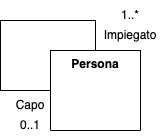
\includegraphics[scale=0.7]{img/riflessiva.png}
    \caption{Esempio di associazione riflessiva.}
\end{figure}

\newpage
\subsubsection{Aggregazione e Composizione}

L'\textbf{\textcolor{cyan}{aggregazione}} e la \textbf{\textcolor{cyan}{composizione}}
sono tipi di relazioni in cui viene specificato che un oggetto di una classe \emph{fà parte} di un oggetto
di un'altra classe. L'\emph{aggregazione} è meno forte come relazione, quindi si verifica quando le \emph{\textcolor{MidnightBlue}{classi parte}} hanno un
significato anche senza la presenza della \emph{\textcolor{MidnightBlue}{classe tutto}}. Nella \emph{composizione}, invece, la \emph{classe parte} ha un senso solo
se legata alla \emph{classe tutto}.

\begin{figure}[h]
    \centering
    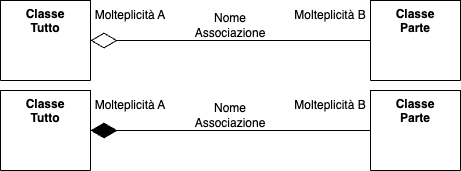
\includegraphics[scale=0.7]{img/aggrecomp.png}
    \caption{Sopra \emph{aggregazione}, sotto \emph{composizione}.}
\end{figure}

\subsubsection{Generalizzazione}
Consiste in una relazione tra una classe più generica e una più specializzata: la classe specializzata o
\emph{\textcolor{cyan}{sottoclasse}} eredita tutte le caratteristiche della \emph{\textcolor{cyan}{superclasse}}, può aggiungerne delle altre, e
può ridefinire delle \emph{operazioni}.

In questa relazione vale il \emph{Principio di Sostituzione di Liskov} \footnote{\url{https://it.wikipedia.org/wiki/Principio_di_sostituzione_di_Liskov}},
ovvero un oggetto della classe specializzata può essere usato al posto di un oggetto della superclasse.

\begin{figure}[h]
    \centering
    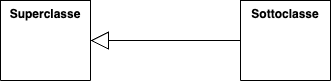
\includegraphics[scale=0.7]{img/generalizzazione.png}
\end{figure}

\newpage
\subsubsection{Classi Astratte}
Le \textbf{\textcolor{cyan}{classi astratte}} definiscono delle classi che non sono implementate completamente.

\begin{figure}[h]
    \centering
    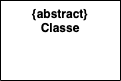
\includegraphics[scale=0.7]{img/abstract.png}
\end{figure}

\subsubsection{Interfacce}
Le \textbf{\textcolor{cyan}{interfacce}} si usano in fase di \emph{progettazione} per definire
delle classi con solo operazioni e senza attributi.

\begin{figure}[h]
    \centering
    
\includegraphics[scale=0.7]{img/interface.png}
\end{figure}

\paragraph{Nota Bene} Sia le \emph{interfacce} che le \emph{classi astratte} non possono essere istanziate, ma si utilizzano
nelle \emph{\textcolor{cyan}{gerarchie}} per definire la "\emph{struttura}" di classi più complete.

\subsubsection{Dipendenze}
La dipendenza è una relazione in cui le classi hanno un ruolo di
\emph{\textcolor{cyan}{cliente}} e di \emph{\textcolor{cyan}{fornitore}}. Questo avviene quando
un parametro di un'operazione della classe \emph{cliente} è un oggetto della classe \emph{fornitore}, o se un'operazione
del \emph{cliente} restituisce o crea dinamicamente un oggetto del tipo del \emph{fornitore}.

\begin{figure}[h]
    \centering
    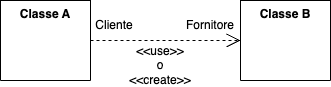
\includegraphics[scale=0.7]{img/dipendenza.png}
\end{figure}

\subsubsection{Classi Associazione}
Un'associazione può avere dei propri attributi, rappresentati con una \textbf{\textcolor{cyan}{classe associazione}}.
Per ogni coppia di classi, può esistere solo una \emph{classe associazione}.

\begin{figure}[h]
    \centering
    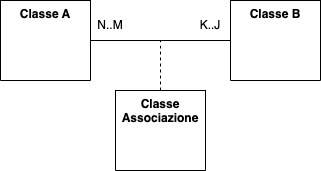
\includegraphics[scale=0.7]{img/classeass.png}
\end{figure}

\subsubsection{Classi di Analisi}
Le \textbf{\textcolor{cyan}{classi di analisi}} corrispondono ai concetti
concreti del dominio, per esempio i termini del glossario. Queste classi hanno un numero
ridotto di \emph{\textcolor{cyan}{funzionalità}} e durante la loro definizione occorre
evitare di:
\begin{itemize}
    \item Definire classi "\emph{\textcolor{cyan}{onnipotenti}}".
    \item Definire classi che in realtà sono delle \emph{\textcolor{cyan}{funzioni}}.
    \item Definire delle \emph{\textcolor{cyan}{gerarchie}} troppo profonde (più di 3 livelli).
    \item Specificare troppo i \emph{\emph{\textcolor{cyan}{tipi}}} e i \emph{\emph{\textcolor{cyan}{valori}}} degli \emph{attributi}.
\end{itemize}
Inoltre le \emph{operazioni} e gli \emph{attributi} vanno indicati solo quando sono veramente utili.

Le principali tecniche di definizione delle \emph{classi di analisi} sono:
\begin{itemize}
    \item \textcolor{cyan}{Data Driven}: durante la \emph{fase di analisi}, si identificano tutti i dati del sistema e si dividono
        in classi.
        \item \textcolor{cyan}{Responsibility Driven}: durante la \emph{fase di progettazione} si identificano le operazioni e si dividono in classi.
\end{itemize}
L'analisi {\textcolor{cyan}{nome-verbo}} consiste nell'associare ai \emph{\textcolor{cyan}{sostantivi}} le classi e gli attributi, mentre ai
\emph{\textcolor{cyan}{verbi}} le operazioni. Successivamente si individuano le relazioni fra le classi. Utilizzando questo
tipo di approccio occorre prestare attenzione ai casi di sinonimia per evitare di definire classi inutili; e bisogna saper individuare
le classi nascoste del dominio, cioè quelle che non vengono mai menzionate esplicitamente.

\newpage
\subsubsection{Diagramma degli Oggetti}
\begin{wrapfigure}{l}{0.\textwidth}
    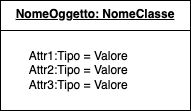
\includegraphics[scale=0.7]{img/diagrammaoggetti.png}
\end{wrapfigure}
In questo caso, un collegamento tra \emph{oggetti} è un'\textbf{\textcolor{cyan}{istanza d'associazione}}, non ha un nome
ma si possono indicare i ruoli. Inoltre non esiste la molteplicità, in quanto è sempre $1$ a $1$.
        \newline
\subsection{Diagramma delle Attività}
Sono utili per descrivere delle \textcolor{cyan}{attività} relative a un qualsiasi \emph{oggetto} o \emph{classe}, ovvero un insieme di azioni che possono essere \emph{sequenziali},
\emph{condizionali}, \emph{concorrenti} e \emph{iterative}.

Si usano sia nella fase di \emph{analisi} per modellare un processo o un caso d'uso,
ma anche per descrivere l'\emph{operazione} di una classe o per modellare un algoritmo in
fase di \emph{testing}.

Il contenuto di un'attività è un \emph{grafo diretto} in cui i \textcolor{cyan}{nodi} sono
le \emph{azioni} o i \emph{nodi di controllo}, mentre gli \textcolor{cyan}{archi} sono i possibili
percorsi percorribili per l'attività.

\begin{figure}[h]
    \centering
    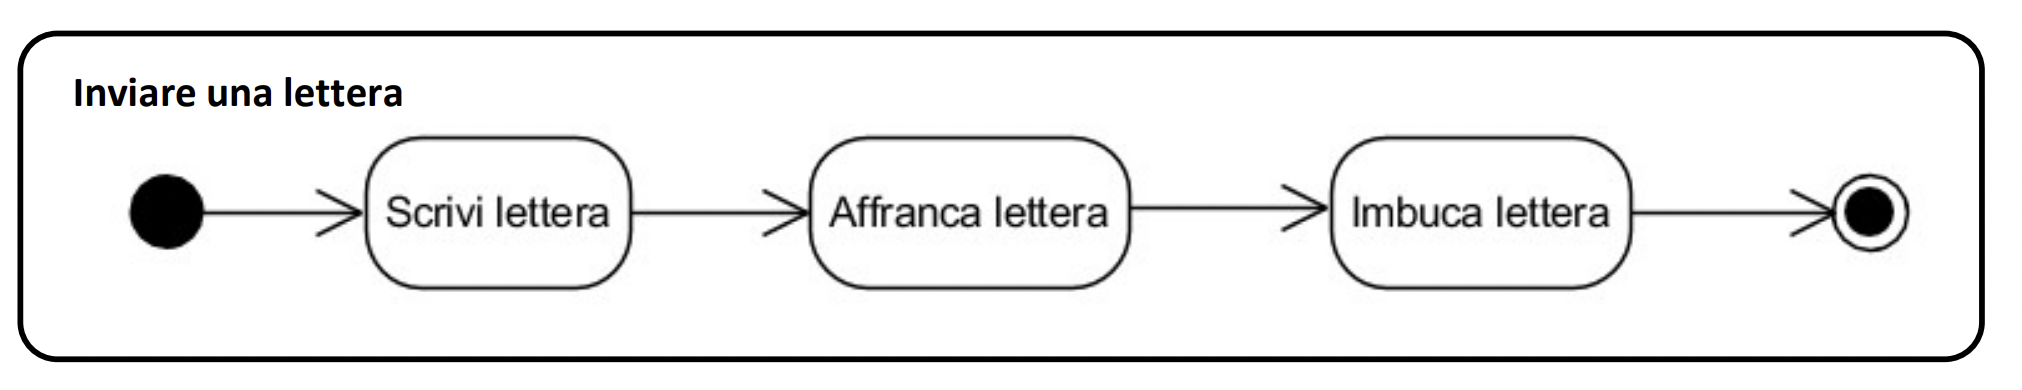
\includegraphics[scale=0.34]{img/azione.png}
\end{figure}

\paragraph{\textcolor{cyan}{Azioni}} È importante sottolineare che le azioni devono essere
\textbf{\textcolor{cyan}{atomiche}}, cioè \underline{non} interrompibili.
Inoltre per ogni azione ci può essere solo una freccia entrante e una uscente.
Quando un'azione è giunta al termina avviene una transazione automatica chiamata
\textbf{\textcolor{cyan}{token}} che porta all'azione successiva.

\begin{figure}[h]
    \centering
    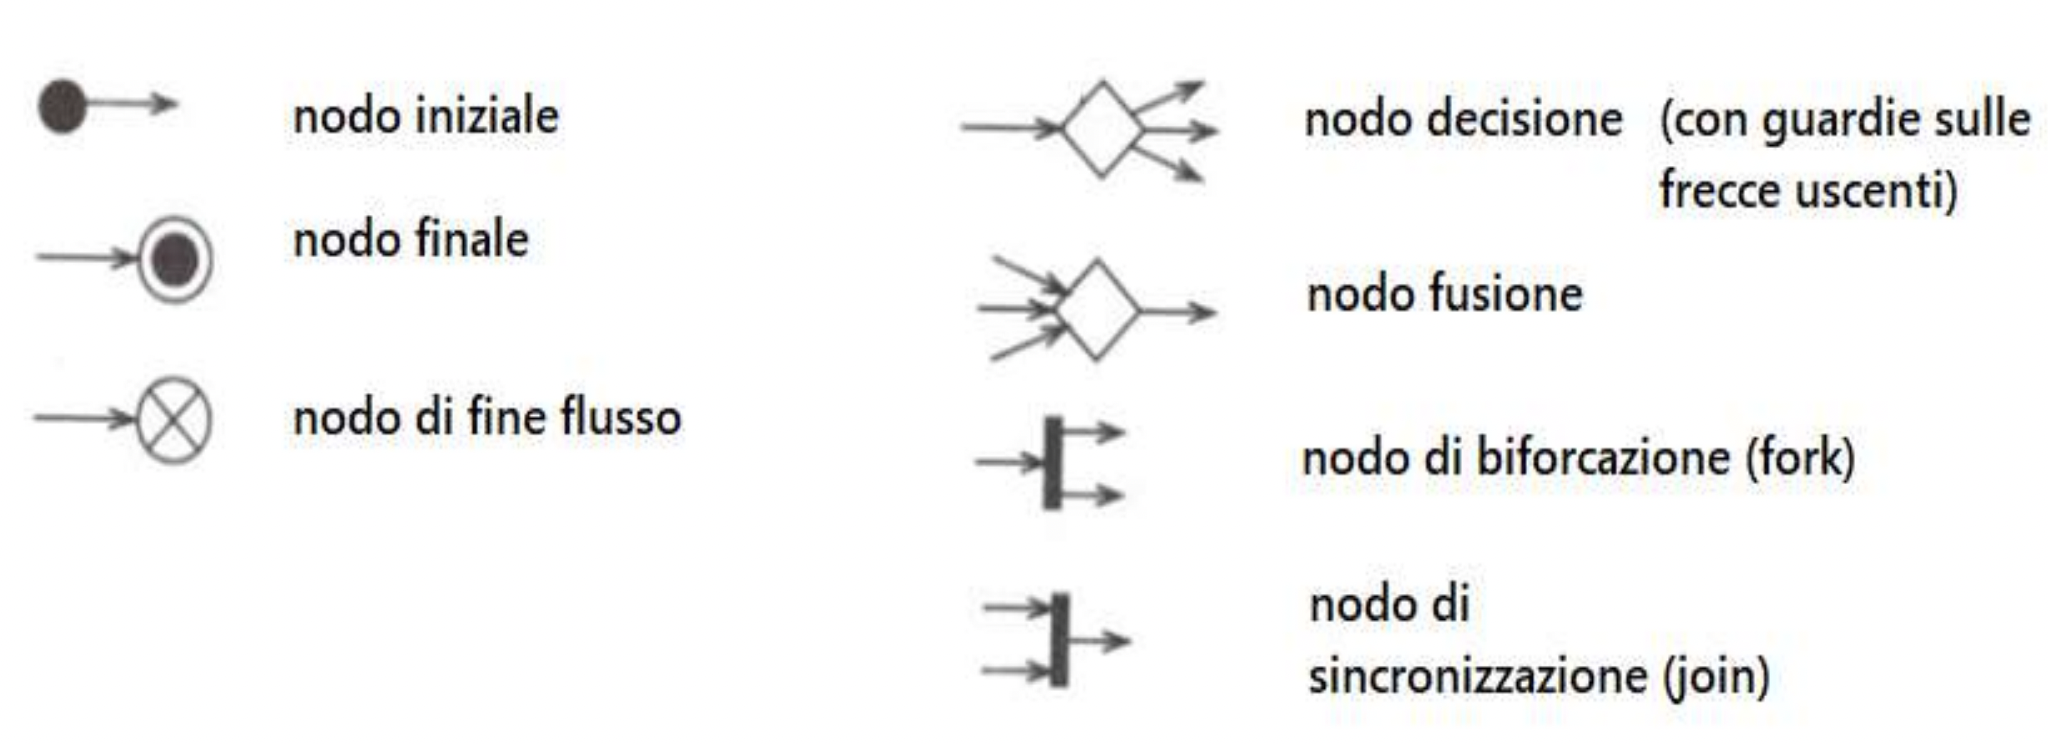
\includegraphics[scale=0.30]{img/nodidecisione.png}
    \caption{Nodi di Controllo}
\end{figure}

\paragraph{\textcolor{cyan}{Nodi di Decisione}} Un nodo di decisione deve poter coprire tutti i casi
possibili, in modo che il \emph{\textcolor{cyan}{token}} non possa bloccarsi. Opzionalmente le \emph{guardie}
possono essere \emph{\textcolor{cyan}{mutualmente esclusive}}.
Inoltre, dato un \emph{nodo decisione} non è obbligatoria la presenza di un \emph{nodo fusione}.

Le \emph{guardie} si scrivono sempre tra parentesi \verb|[]|.

\paragraph{\textcolor{cyan}{Fork \& Join}} La \emph{fork} moltiplica i token, producendone
uno per ogni uscita. La \emph{join} invece attende un token per ogni freccia entrante e, quando li consuma tutti, ne esce
solo uno. Come per i nodo di decisione non è necessaria una \emph{join} per ogni \emph{fork}.

\paragraph{\textcolor{cyan}{Nodo di Fine Attività}} Quando un qualsiasi token raggiunge questo nodo
tutta l'attività termina. Solo su questi nodi, e su quelli di \emph{fine flusso}, possono essere presenti più
archi entranti; ciò sta a significare che il primo token che arriva termina l'attività.

\paragraph{\textcolor{cyan}{Nodo di Fine Flusso}} Questo tipo di nodo non termina l'attività, ma consuma il token.

\subsubsection{Segnali \& Eventi}

\begin{itemize}
    \item Accettazione di un evento esterno.
        \begin{figure}[h]
            \centering
            
\includegraphics[scale=0.30]{img/accettaevento.png}
        \end{figure}
    \item Invio di un segnale. L'invio di segnali è \textcolor{cyan}{\underline{asincrono}}, cioè non blocca l'attività.
        \begin{figure}[h]
            \centering
            
\includegraphics[scale=0.30]{img/mandasegnale.png}
        \end{figure}    
    \item Accettazione di un evento temporale.
        \begin{figure}[H]
            \centering
            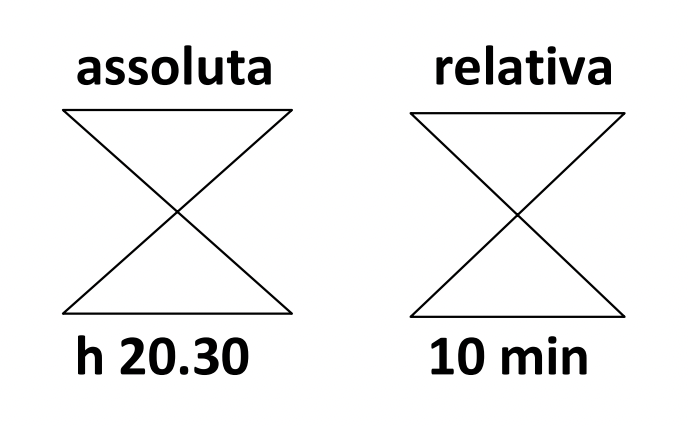
\includegraphics[scale=0.30]{img/tempo.png}
        \end{figure}
\end{itemize}

Per gli eventi \textcolor{cyan}{esterni} e \textcolor{cyan}{temporali}, gli archi entranti non sono
necessari, quindi in questo caso quando si verifica quel determinato evento viene generato un token.
Se invece gli archi entranti sono presenti, quando arriva il token questo attende che l'evento esterno si verifichi.

A differenza delle \textcolor{cyan}{azioni} che si usano quando le attività sono effettuate
dalle entità di cui si sta descrivendo il comportamento, mentre i \textcolor{cyan}{segnali} e gli
\textcolor{cyan}{eventi} si usano quando si comunica con un'entità esterna.

\subsubsection{Sotto-Attività}

Un diagramma può contenere il riferimento a delle attività secondarie, rappresentate
come un'azione ma con in più il simbolo di un "rastrello".

\begin{figure}[h]
    \centering
    \includegraphics[scale=0.45]{img/sottoattività.png}
\end{figure}

\subsubsection{Partizioni}

Le \textbf{\textcolor{cyan}{partizioni}} permettono di dividere le azioni, assegnandole
all'entità che ne è responsabile.
        \subsection{Macchina a Stati}
È un grafo "\emph{stati-transizioni}" che permette di descrivere il comportamento delle istanze di una classe.
A differenza dei \emph{diagrammi delle attività} dove l'obbiettivo è mettere in ordine un insieme di azioni, qui viene
mostrata l'evoluzioni degli oggetti in risposta a determinati eventi.
\newline\newline
Ogni \textcolor{cyan}{transizione} avviene al verificarsi di un determinato evento interno, rappresentato da un'\emph{operazione}
della classe; oppure tramite messaggi inviati da altri oggetti.

In una \emph{transizione}, gli \emph{\textcolor{cyan}{eventi}} possono essere accompagnati
anche da una \emph{\textcolor{cyan}{condizione}} e da una sequenza di azioni.

\begin{figure}[h]
    \centering
    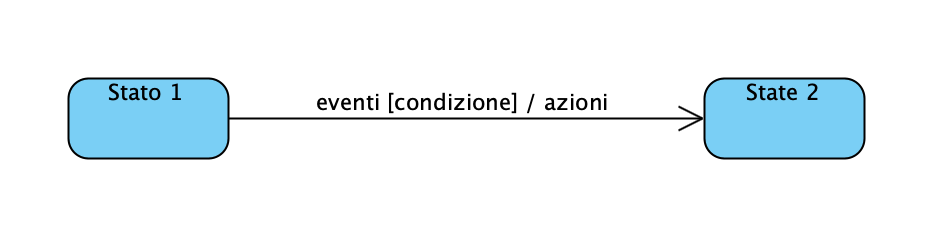
\includegraphics[scale=0.7]{img/machinediagram.png}
\end{figure}

La semantica è la seguente: se si verifica almeno uno degli eventi, e vale la condizione, si eseguono
tutte le azioni e si passa nell'altro stato.

\subsubsection{Eventi}

Le \emph{transizioni} possono essere \emph{non deterministiche}, cioè da uno stato ci possono
essere più transizioni con lo stesso evento.

Gli eventi possono classificarsi in:
\begin{itemize}
    \item Eventi di \textcolor{cyan}{operazione} o \textcolor{cyan}{segnale}: \verb|op(a: T)|. Ovvero la transizione
        è abilitata quando riceve un segnale o avviene una chiamata di metodo con parametri \verb|a| e tipo \verb|T|.
    \item Eventi di \textcolor{cyan}{variazione}: \verb|when(exp)|. La transizione è abilitata quando \verb|exp| diventa vera.
    \item Eventi \textcolor{cyan}{temporali}: \verb|after(time)|. La transizione è abilitata dopo che l'oggetto è stato fermo per
        un tempo \verb|time| in quello stato.
\end{itemize}

\paragraph{\textcolor{cyan}{Entry}} Anche chiamata \emph{azione di entrata}, viene eseguita all'ingresso di uno stato.
\paragraph{\textcolor{cyan}{Exit}} Anche chiamata \emph{azione di uscita}, viene eseguita quando si esce da uno stato.
\paragraph{\textcolor{cyan}{Transizione Interna}} Risposta a un determinato evento, ma si rimane nello stesso stato.
\paragraph{\textcolor{cyan}{Do-Activity}} Azione eseguita in continuazione finchè l'oggetto si trova in quello stato.
A differenza delle altre \emph{azione} che sono \emph{atomiche}, queste consumano del tempo e possono essere interrotte, ad esempio
quando si esce dallo stato.

\begin{figure}[h]
    \centering
    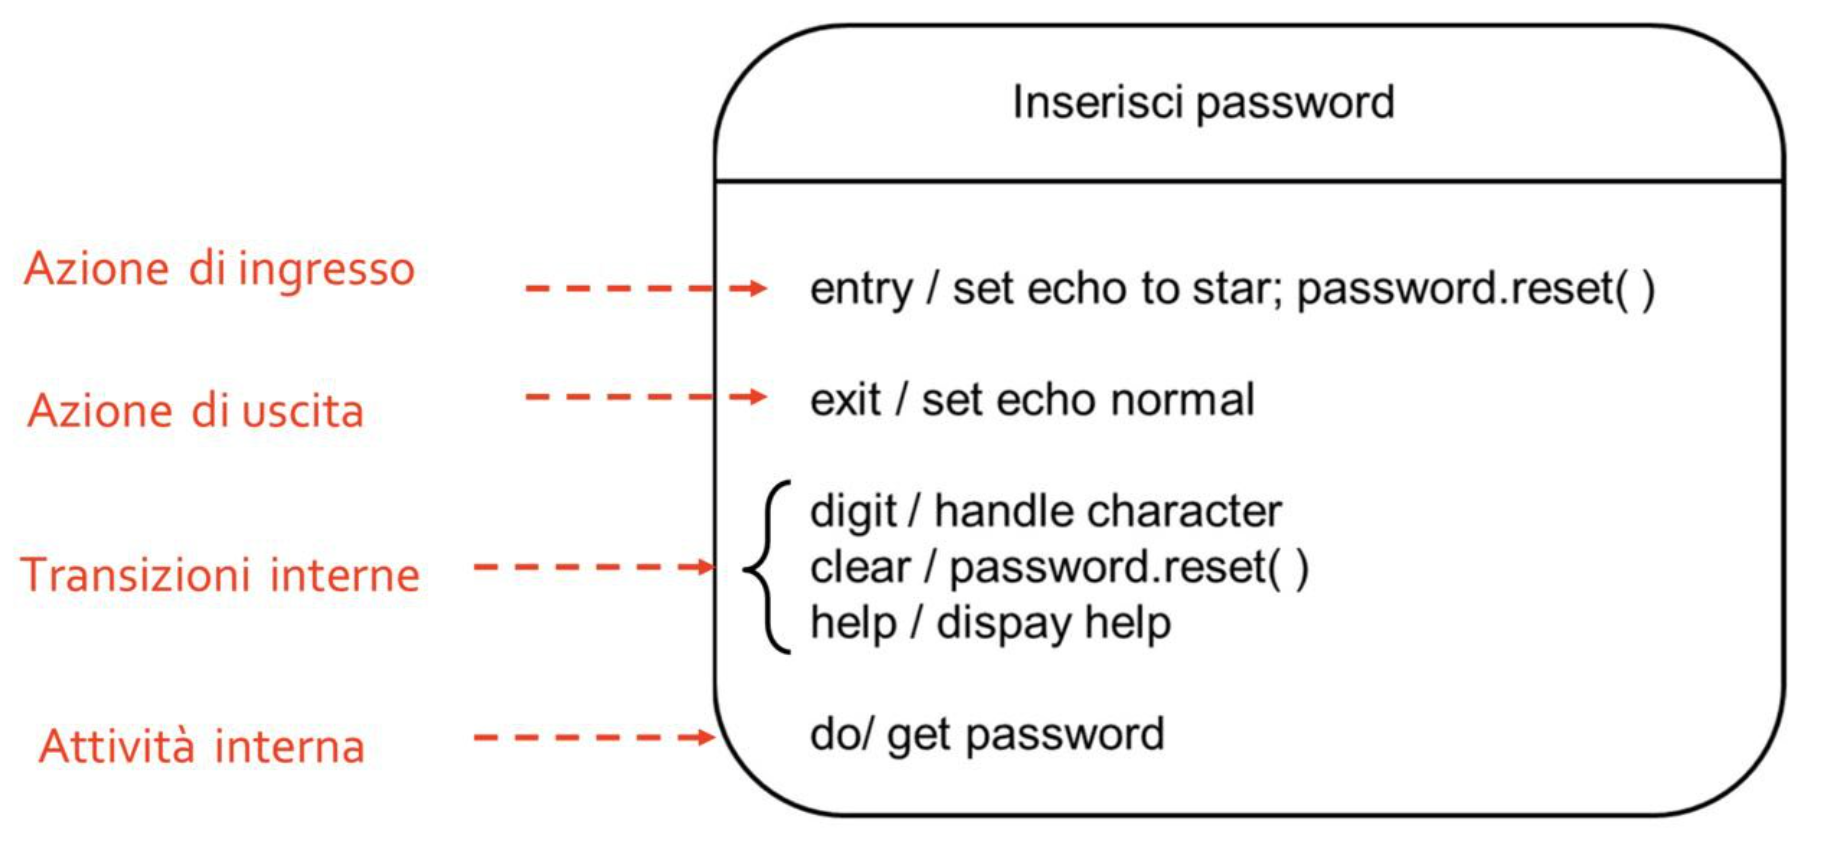
\includegraphics[scale=0.37]{img/entry.png}
\end{figure}

\newpage

\subsubsection{Stato Composito Sequenziale}
Consiste nell'avere uno stato che contiene un'altra \emph{macchina a stati}.
Quando una transizione entrante nello \emph{\textcolor{cyan}{stato composito}} termina sul bordo, vuol
dire che si prosegue a partire dallo \emph{stato iniziale} dello \emph{stato composito}. Altrimenti la transizione
può avere come \emph{target} anche uno stato interno.
Le transizioni di uscita, invece, possono anch'esse partire dal bordo, in tal caso
significa che ci si può andare da qualsiasi stato interno, altrimenti quelle che partono da un singolo stato interno
sono possibili solo da esso. Esiste anche una transizione d'uscita speciale chiamata di \textcolor{cyan}{completamento},
dalla quale ci si può passare solo una volta arrivati nello stato finale dello stato composito.

\begin{figure}[H]
    \captionsetup{justification=centering}
    \centering
    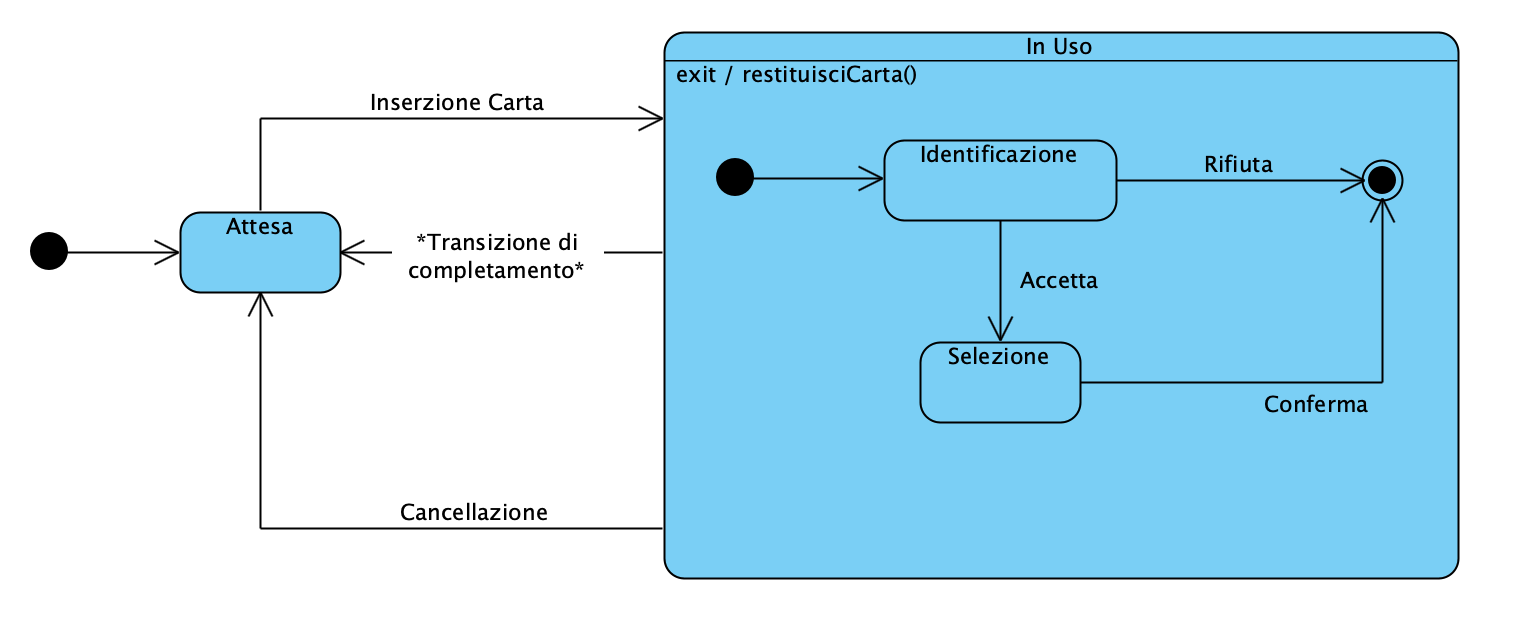
\includegraphics[scale=0.45]{img/statocompositoseq.png}
    \caption{Esempio di macchina a stati che descrive l'uso di un sistema di pagamento con stato composito sequenziale.}
\end{figure}

\newpage

\subsubsection{Stato Composito Parallelo}
Nello \emph{stato composito} abbiamo più sottostati che si eseguono in modo
parallelo. Una transizione entrante sul bordo attiva tutti gli stati iniziali.
La \emph{transizione di completamento} può avvenire solo se si è arrivati in tutti gli stati finali.
Mentre, una transizione di uscita che parte dal bordo è raggiungibile da un qualunque stato interno e fà uscire da \textbf{tutti}
i sottostati. Anche un transizione che parte da un singolo stato interno fà uscire da tutti i sottostati e può avvenire solo se ci
si trova in quel determinato stato.

\begin{figure}[H]
    \centering
    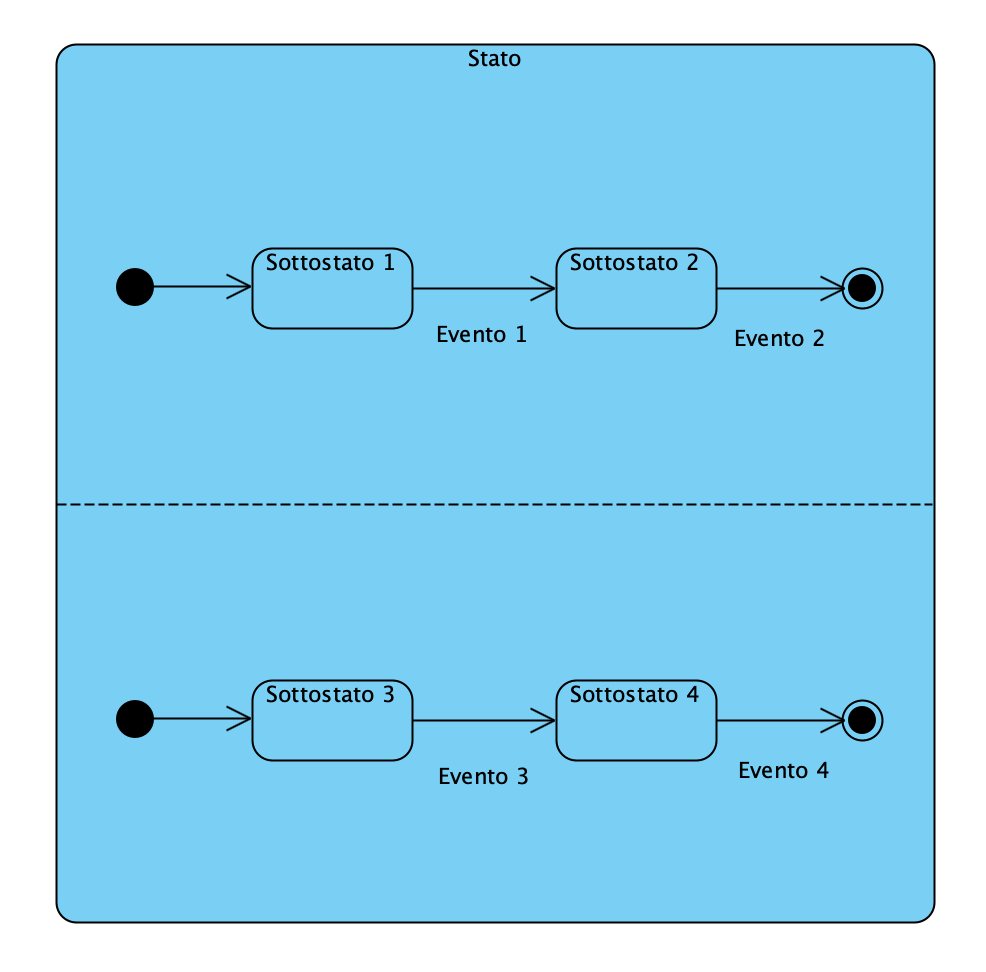
\includegraphics[scale=0.6]{img/statoparallelo.png}
\end{figure}

\subsubsection{Sottomacchine}
Le \textcolor{cyan}{sottomacchine} si usano quando si vuole rappresentare
uno stato composito in un diagramma a parte, in modo da poterlo riusare in più contesti.
La \emph{sottomacchina} ha un nome che ne definisce il \verb|Tipo| e le sue istanze
si indicano con \verb|Nome Istanza: Tipo|.

\paragraph{\textcolor{cyan}{Entry \& Exit Points}} Sono dei nodi che servono per poter collegare le transizioni
della macchina principale con la sottomacchina.

\begin{figure}[H]
    \centering
    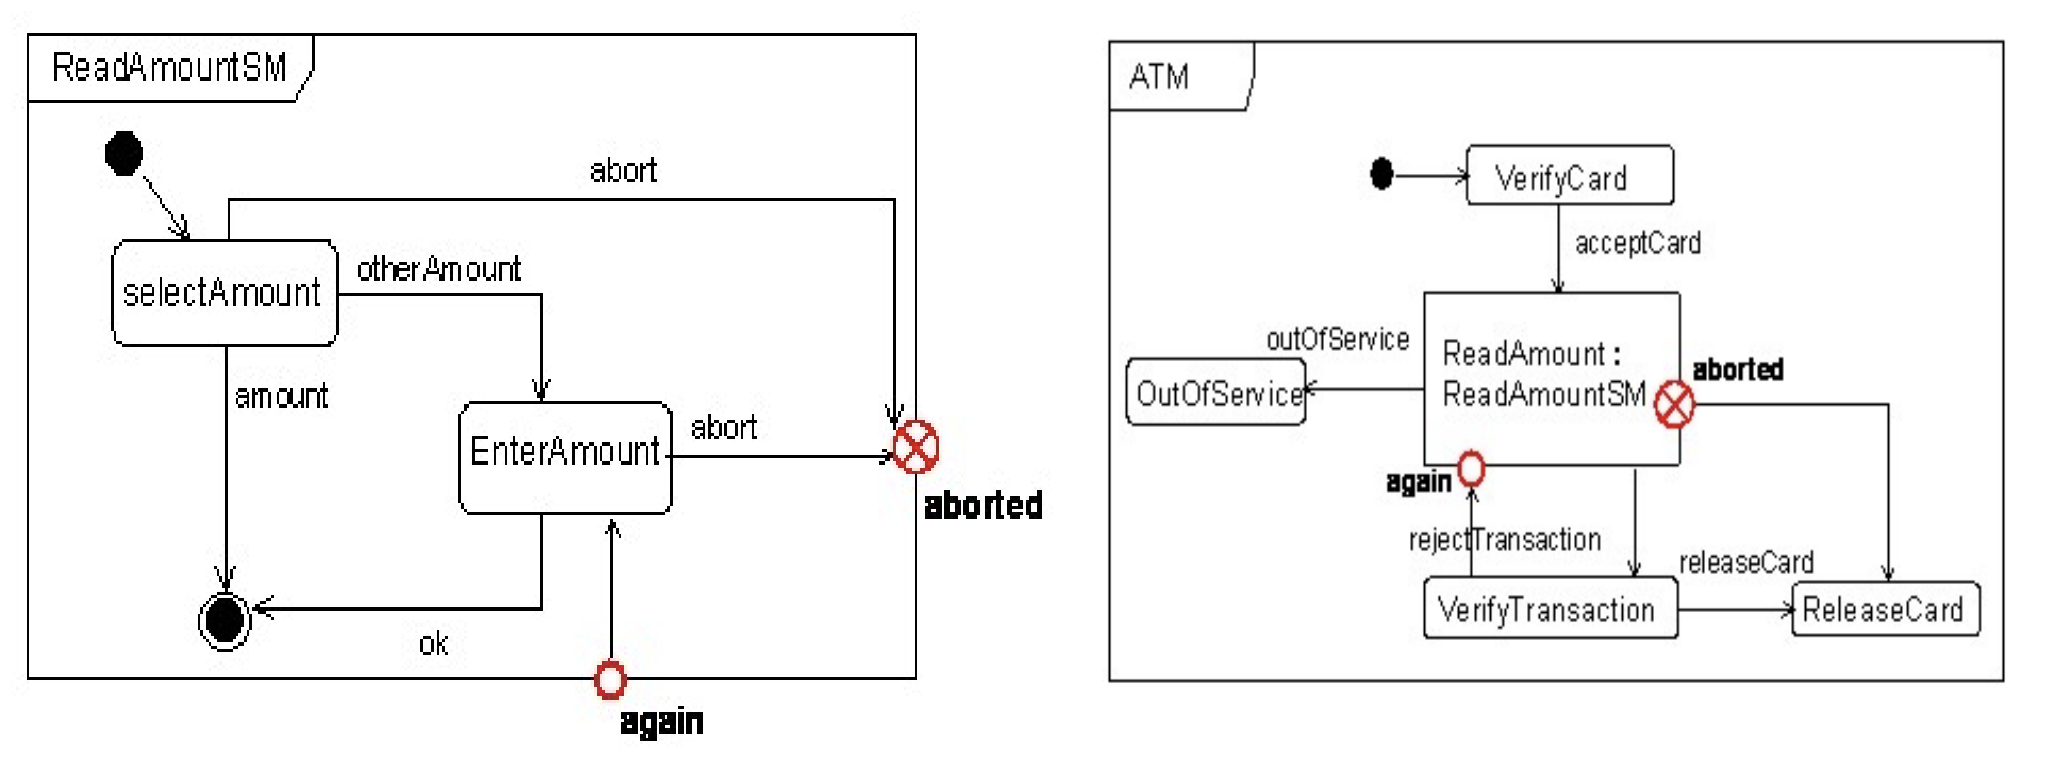
\includegraphics[scale=0.33]{img/sottomacchine.png}
\end{figure}

In questo caso le \emph{transizioni di completamento} possono scattare anche quando si arriva in un \emph{exit point}. 

\subsubsection{Pseudostati}

\paragraph{\textcolor{cyan}{Giunzione}} Uno \emph{pseudostato} da cui possono entrare e/o uscire due o più transizioni.
Se sono presenti condizioni, queste sono valutate in modo \textcolor{cyan}{statico}, quindi prima che avvengano gli eventi interessati.
Inoltre, se le condizioni non coprono tutti i casi, l'evento può essere ignorato e si rimane in quello stato.

\begin{figure}[H]
    \centering
    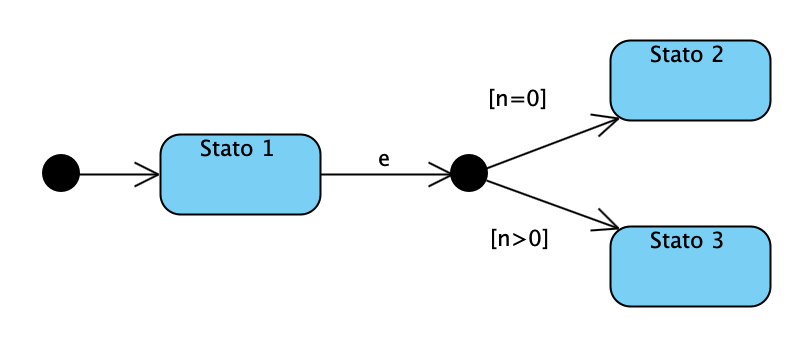
\includegraphics[scale=0.7]{img/giunzione.png}
\end{figure}

\paragraph{\textcolor{cyan}{Decisione}}

A differenza delle \emph{\textcolor{cyan}{giunzioni}}, questo sono valutate \textcolor{cyan}{dinamicamente}, quindi dopo che avvengono
gli eventi; e devono coprire tutti i casi possibili. Ovviamente un'altra differenza con le \emph{giunzioni} è che in questo caso la transizione
entrante può essere solo \underline{una}.

\begin{figure}[H]
    \captionsetup{justification=centering}
    \centering
    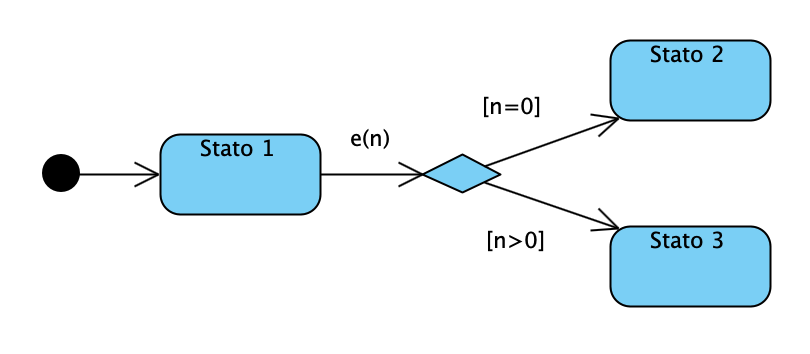
\includegraphics[scale=0.7]{img/choice.png}
    \caption{In questo esempio bisogna avere garanzia che $n \geq 0$.}
\end{figure}

\paragraph{\textcolor{cyan}{Storia}}

Lo stato \emph{\textcolor{cyan}{history}} permette di memorizzare lo stato della macchina
quando viene \emph{interrotta} o \emph{spenta}. La transizione entrante nello stato \emph{history}, invoca il
ripristino dello stato precedente, mentre se c'è una transizione uscente, questa indica lo stato in cui passare nel caso
in cui la macchina non sia ancora stata mai interrotta, quindi quando lo stato \emph{history} è vuoto.

\begin{figure}[H]
    \captionsetup{justification=centering}
    \centering
    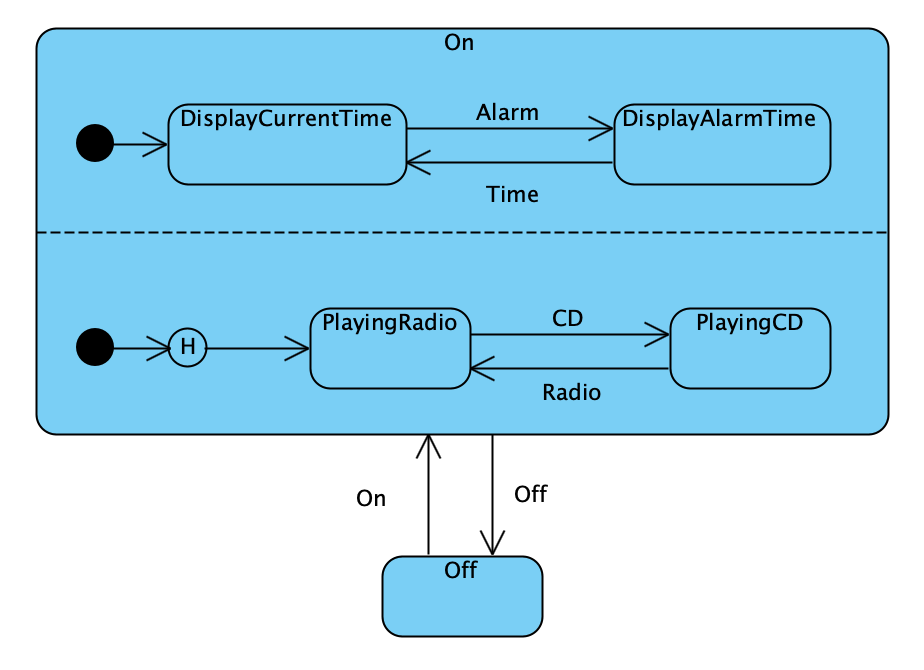
\includegraphics[scale=0.7]{img/history.png}
    \caption{In questo esempio di funzionamento di un autoradio, la prima volta che si accenderà verrà riprodotta in automatico una stazione radio.}
\end{figure}
        \section{Architetture Software}
La \emph{\textcolor{cyan}{progettazione}} è la fase che segue la \emph{specifica} e
precede la \emph{codifica}. Descrive in che modo deve essere realizzato il progetto. Il suo
prodotto si chiama \emph{architettura}.

Esistono due tipi di \emph{progettazione}:
\begin{itemize}
    \item Progettazione di \textcolor{cyan}{alto livello}: lo scopo è identificare
        e scomporre il sistema in tanti piccoli sottosistemi e definire le loro inter-connessioni.
    \item Progettazione di \textcolor{cyan}{dettaglio}: si decide come ogni singolo \emph{sottosistema} deve
        essere realizzato.
\end{itemize}

Quindi l'\textcolor{cyan}{architettura} di un sistema software è la
struttura del sistema costituita dalle sue parti e dalle relazioni fra esse,
più le loro proprietà visibili all'esterno. Vengono considerati anche gli aspetti
\emph{\textcolor{cyan}{non funzionali}}.

Durante questa fase il sistema viene analizzato attraverso tre punti di vista:
\begin{itemize}
    \item Vista \textbf{\textcolor{cyan}{Comportamentale}} o \emph{component-and-connector}: questa vista descrive il sistema trattandolo
        come composizione di altri software. Quindi si specificano tutte le componenti (i software), che presentano delle \emph{interfacce},
        successivamente si descrivono le caratteristiche dei \emph{connettori} che collegano le varie componenti. Infine si
        analizza la struttura del sistema in esecuzione, infatti questa vista è molto utile per analizzare la qualità e le prestazioni del software e per documentare
        lo stile dell'architettura. 
    \item Vista \textbf{\textcolor{cyan}{Strutturale}}: permette di descrivere la struttura del sistema vedendolo
        come un insieme di \emph{classi} e/o \emph{packages}. È utile per analizzare le dipendenza tra le \emph{classi}/\emph{packages}
        e per progettare i test di \emph{unità} e di \emph{integrazione}.
    \item Vista \textbf{\textcolor{cyan}{Logica}} o di \emph{deployment}: descrive l'allocazione del software su più ambienti di esecuzione.
\end{itemize}

\subsection{Vista Comportamentale}

\begin{definition}[Componente]
    Una \textbf{\textcolor{cyan}{componente software}} è un'unità software indipendente
    e che può essere riusata da altri componenti. Incapsula un insieme di funzionalità e/o di
    dati di un sistema, restringendo l'accesso ad essi tramite la definizione di \emph{iterfacce}.
\end{definition}

\begin{figure}[H]
    \centering
    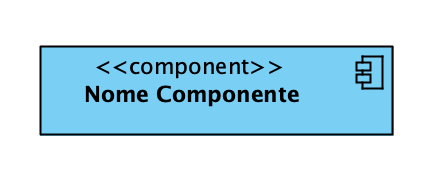
\includegraphics[scale=0.8]{img/component.png}
\end{figure}

\begin{definition}[Porti]
    I \textbf{\textcolor{cyan}{porti}} identificano i punti di interazione di un componente, ogni componente ne ha uno
    per ogni connessione che ha con altri componenti. Un \emph{porto} può richiedere una o più interfacce dello stesso tipo.
\end{definition}

\begin{figure}[H]
    \centering
    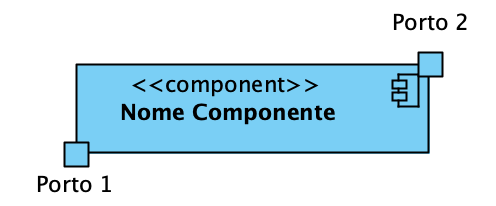
\includegraphics[scale=0.8]{img/porti.png}
\end{figure}

Le \emph{\textcolor{cyan}{interfacce}} possono essere rappresentate in modo esteso o in modo sintetico mediante l'uso
di \emph{forchette} (quando viene richiesta un'interfaccia) o \emph{lollipop} (quando l'interfaccia è fornita).

\begin{figure}[H]
    \centering
    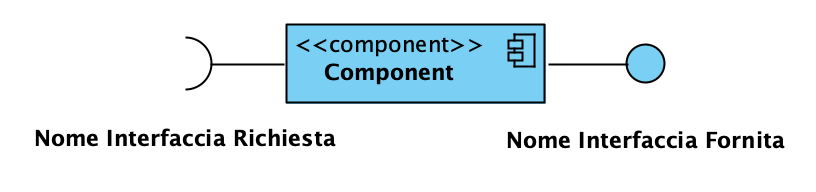
\includegraphics[scale=0.8]{img/lollipop.png}
    \caption{Modo Sintetico}
\end{figure}

\begin{figure}[H]
    \centering
    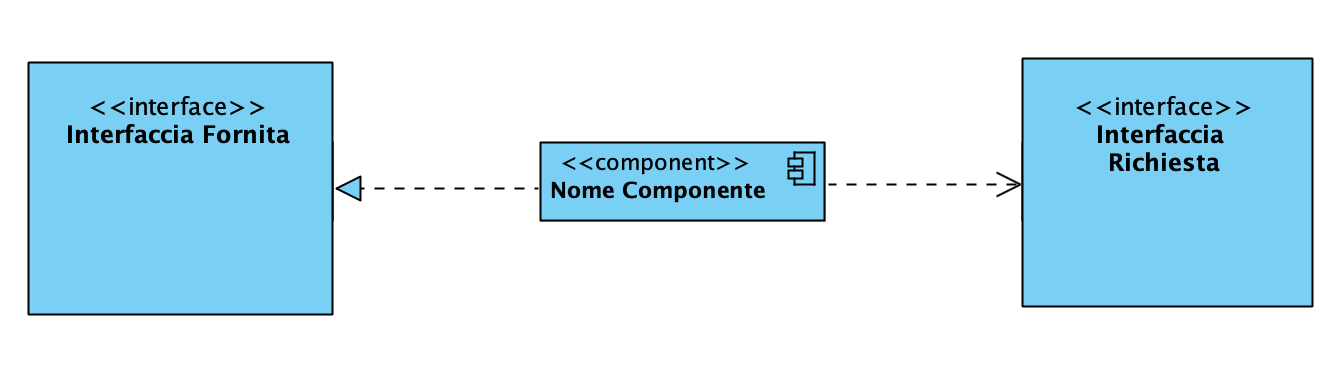
\includegraphics[scale=0.5]{img/interfacce.png}
    \caption{Modo Esteso}
\end{figure}

\begin{definition}[Connettori]
    I \textbf{\textcolor{cyan}{connettori}} sono i canali di comunicazione che collegano i \emph{porti} fra componenti
    diverse. Sul connettore è possibile indicare il \emph{protocollo di comunicazione} utilizzato fra \verb|<<...>>|.
\end{definition}

\subsubsection{Stili Architetturali}
\begin{definition}[Stile]
    Uno \textbf{\textcolor{cyan}{stile}} è una proprietà dell'architettura che ne caratterizza una famiglia con caratteristiche
    e interazioni fra componenti comuni.
\end{definition}

\paragraph{\textcolor{cyan}{Pipe \& Filter}}
Le componenti sono di tipo \emph{filtro}, ovvero effettuano delle trasformazioni sui dati
che provengono dai porti d'ingresso e li mandano sui porti d'uscita. I connettori, invece, sono di tipo
\emph{pipe}, ovvero un canale di comunicazione unidirezionale e che preserva l'ordine dei dati che entrano e che escono.

\paragraph{\textcolor{cyan}{Client-Server}}
Il sistema è formato da componenti che si comportano da \emph{client} e altri da \emph{server}.
Il client si connette a un server tramite un porto per richiedere un servizio, il server può ricevere connessioni da parte
di più client.

\paragraph{\textcolor{cyan}{Master-Slave}} È un caso particolare del
modello \emph{client-server}, in cui lo \emph{slave} (il server) può servire
un solo \emph{master} (client).

\paragraph{\textcolor{cyan}{Peer-to-Peer}} Tutti i componenti agiscono sia da client che da server, quindi nella
rappresentazione ci sarà un solo componente.

\paragraph{\textcolor{cyan}{Publish-Subscrive}} I componenti interagiscono tra loro
tramite l'annuncio di eventi, una componente può svolgere sia il ruolo di \emph{Publisher} (produttore di eventi) che di
\emph{Subscriber} (consumatore di eventi). Questo stile può coinvolgere anche un
intermediario chiamato \emph{broker}, che permette alle altre componenti di non interagire direttamente
fra loro e quindi di non essere consapevole delle indentià delle altre.

\paragraph{\textcolor{cyan}{Model-View-Controller}} Permette di isolare il \emph{\textcolor{cyan}{modello}},
ovvero le funzionalità e i dati del sistema, la \emph{\textcolor{cyan}{vista}}, quindi come viene rappresentato il modello, e il 
\emph{\textcolor{cyan}{controllore}}, che riceve l'input ed effettua le chiamate alle operazioni del modello.

\paragraph{\textcolor{cyan}{Coordinatore di Processi}} Prevede l'uso di un componente noto come
\emph{\textcolor{cyan}{coordinatore}}, che conosce la sequenza per realizzare il processo. Una volta ricevuta
la richiesta, chiama le componenti \emph{server} nell'ordine prefissato e successivamente fornisce una risposta.
I server non sono a conoscenza del loro ruolo, ma si limitano solo a fornire un servizio.

\subsection{Vista Strutturale}

Gli elementi di questa vista sono chiamati \emph{\textcolor{cyan}{moduli}}, ed essendo
classi o packages, le relazioni fra essi sono di ereditarietà, dipendenza o composizione.
Un \emph{package} può contenere un insieme di classi e/o di altri packages.

Questo tipo di vista è utile per fornire uno schema del codice e dei file sorgenti, non và utilizzato per le analisi dinamiche,
effettuate con viste \emph{comportamentali} e \emph{logistiche}.

Nelle classi, rispetto alla descrizione del \emph{dominio}, qui si specificano meglio
le loro operazioni.

\subsubsection{Vista Strutturale a Strati}

Gli elementi sono gli \emph{\textcolor{cyan}{strati}}, ovvero un insieme di moduli, che possono essere
raggruppati in \emph{segmenti}, inoltre implementano un'interfaccia pubblica, chiamata \emph{\textcolor{cyan}{macchina virtuale}} per i servizi che offrono.
La relazione fra gli strati è di tipo \verb|<<allowedToUse>>|, è antisimmetrica e non è transitiva.

\subsubsection{Vista Strutturale di Generalizzazione}

Gli elementi sono sempre i moduli, ma la relazione è solo di \emph{generalizzazione}.

\subsection{Vista Logistica}

In questa vista gli elementi possono essere \emph{hardware} (rappresentati da parallelepipedi) come l'ambiente di esecuzione, oppure
\emph{software} (con stereotipo \verb|<<artifact>>|), chiamati \emph{\textcolor{cyan}{artefatti}}, cioè qualsiasi file che viene utilizzato o prodotto
da un software da un sistema generale. Si usa per valutare le prestazioni e per redigere
una guida per l'installazione del software. Le relazioni tra i gli elementi hardware possono essere
connessioni fisiche o protocolli di comunicazione.

\begin{figure}[H]
    \centering
    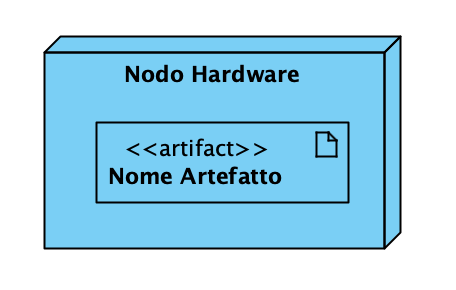
\includegraphics[scale=0.8]{img/architettura.png}
\end{figure}

\paragraph{\textcolor{cyan}{Artefatto}} L'artefatto è una copia di un'implementazione di un componente
che è stata installata su un ambiente di esecuzione. L'artefatto si dice che "\emph{manifesta}" (\verb|<<manifesta>>|) un componente.
        \pagebreak
\section{Diagrammi di Sequenza}
Si usano per descrivere lo scambio di messaggi e dati tra oggetti, indicando
anche la sequenza temporale. Si può usare sia in \emph{fase di analisi} per formalizzare
la \emph{sequenza principale degli eventi} nei casi d'uso, oppure in \emph{fase di progettazione}
per mostrare i messaggi scambiati dalle componenti (e anche attori) nell'architettura.

Gli oggetti e attori sono rappresentati da un rettangolo che indica il ruolo
e/o il tipo (nel caso dell'oggetto). Dal rettangolo parte una linea verticale chiamata \emph{linea di vita}
dell'oggetto: è tratteggiata quando l'entità è inattiva, invece è continua e doppia quando è attiva (nel caso di un attore la sua linea di vita è sempre attiva).

\begin{figure}[H]
    \centering
    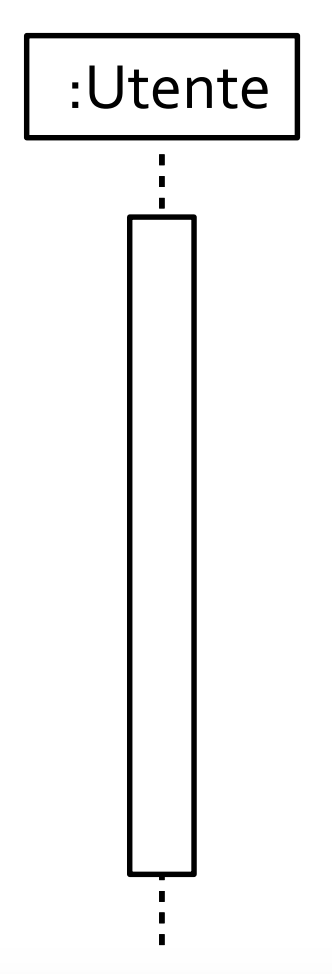
\includegraphics[scale=0.4]{img/sequenza.png}
\end{figure}

\paragraph{\textcolor{cyan}{Messaggi}} I messaggi rappresentano l'invocazione
di \emph{operazioni} o \emph{segnali}, possono essere:
\begin{itemize}
    \item Sincroni (\verb|1|)
    \item Di ritorno (\verb|1.1|)
    \item Asincroni (\verb|2|)
    \item Asincroni con esplicito uso di tempo (\verb|3|)
\end{itemize}

\begin{figure}[H]
    \centering
    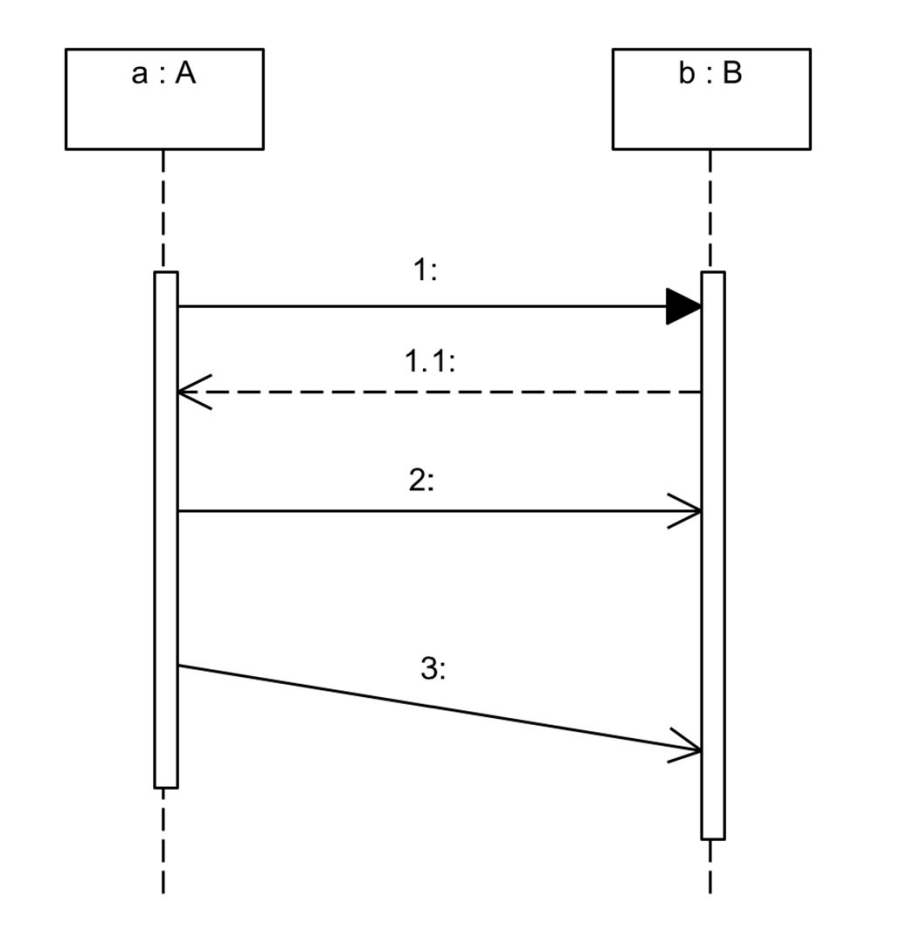
\includegraphics[scale=0.5]{img/messaggi_sequenza.png}
\end{figure}

Inoltre i messaggi presentano la seguente sintassi:

\begin{center}
    \verb|id: attributo = | \\
    \verb|nome_messaggio(arg1, arg2, ..., argN): valore_ritorno|
\end{center}

Le entità possono essere aggiunte e rimosse anche dinamicamente all'interazione.
Per la creazione si indica sulla freccia del messaggio la keyword \verb|<<create>>|.
Per la cancellazione, invece, si pone una $\times$ alla fine della sua linea di vita.


Nella linea di vita è possibile indicare anche vincoli di tempo o durata
per indicare un limite inferiore e/o superiore alla durata di un intervallo.

\paragraph{\textcolor{cyan}{Frame Condizionale}} È possibile dividere
il \emph{frame} del diagramma in più \emph{sottoframe}, ognuno dei quali
può avere una guardia (se non ne ha si assume che sia uguale a \verb|[true]|). In base
alla guardia che è vera (se ce n'è più di una la scelta è non deterministica) si
eseguono le azioni corrispondenti a quel sottoframe.

\paragraph{\textcolor{cyan}{Frame Iterativo}} Un frame può essere ripetuto più volte, si utilizza
la sintassi \verb|loop(min, max)|.

\begin{figure}[H]
    \centering
    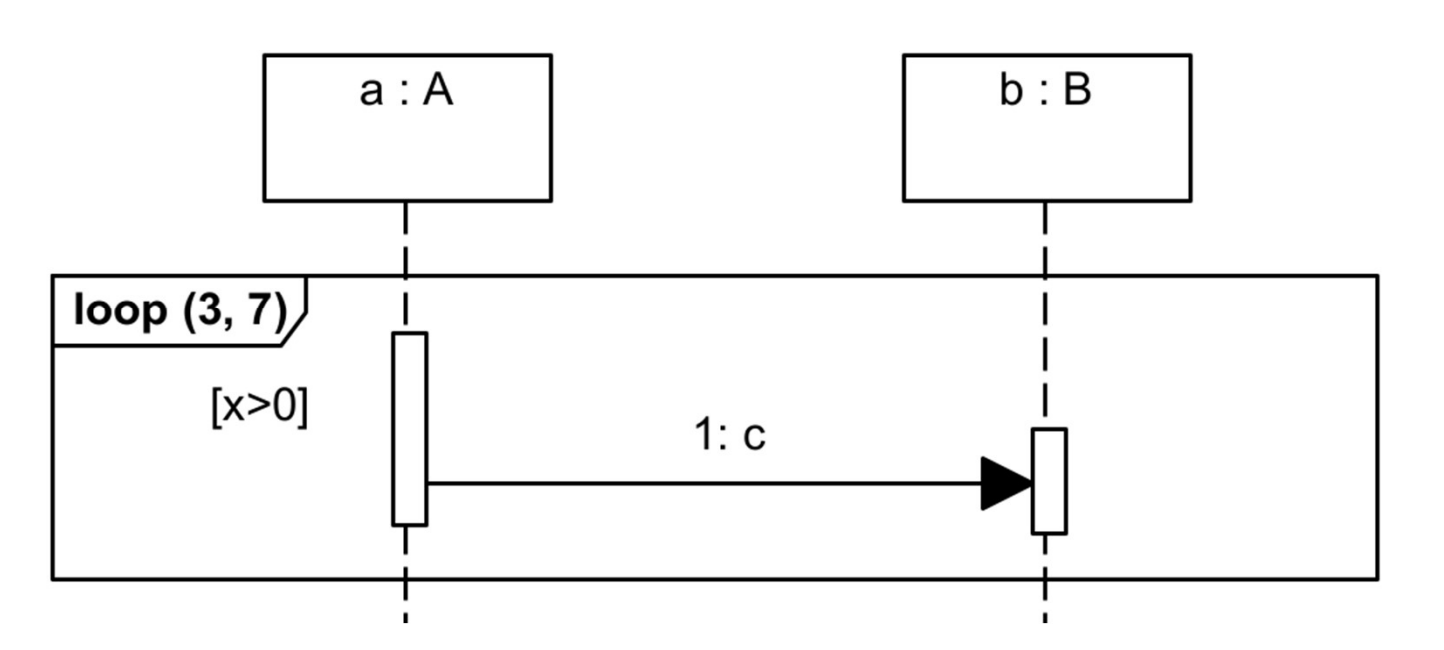
\includegraphics[scale=0.4]{img/frame_iterativo.png}
\end{figure}

\paragraph{Esempi.}

\begin{itemize}
    \item \verb|loop(0, *)[guardia]|: modella il \verb|while(guardia){...}|.
    \item \verb|loop(1, *)[guardia]|: modella il \verb|do{...}while(guardia)|.
    \item \verb|loop(n, n)| o \verb|loop(n)|: modellano un ciclo \verb|for| che và da $0$ a $n$ escluso.
\end{itemize}

\paragraph{\textcolor{cyan}{Frame Condizionale}} Si specifica con la keyword \verb|opt| ed è associato
ad una guardia che, nel caso è vera fà eseguire quel determinato frame.

\paragraph{\textcolor{cyan}{Frame Parallelo}} Le interazioni nei \emph{sottoframe} sono eseguiti
in parallelo (\emph{interleaving}).

\paragraph{\textcolor{cyan}{Ref}} È possibile includere in un frame un'interazione già definita tramite
l'indicatore \verb|ref| e scrivendo il nome del diagramma di sequenza da includere.

\paragraph{\textcolor{cyan}{Gates}} Un \emph{gate} è un punto sul bordo del diagramma a cui è
collegato un messaggio, o in ingresso o in uscita. Ogni gate ha un nome, e si utilizzano principalmente
quando si includono altri diagrammi.

        \newpage

\section{Progettazione Software}
Questa fase risulta molto importante, in quanto si mira a realizzare un software,
che oltre ad essere perfettamente funzionante, deve essere facilmente mantenibile e riusabile in altri sistemi.

Durante la progettazione vengono assegnati i metodi alle classi e si specifica con gli oggetti devono
interagire fra loro per realizzare i casi d'uso. In questa realizzazione si usano i diagrammi di interazione e i \emph{pattern},
e si assegano le \emph{responsabilità} alle classi. Esistono due tipi principali di
responsabilità, quelle di \emph{azione} che definiscono ciò che possono fare gli oggetti, e quelle di \emph{conoscenza} ovvero i dati
a cui hanno accesso direttamente o indirettamente (tramite calcolo).

È importante sottolineare che un \emph{metodo} di una classe non è una \emph{responsabilità}, ma i metodi
vengono implementati per soddisfare le responsabilità.

\subsection{Principi Generali}

\subsubsection{Information Hiding}
Consiste nel separare l'\emph{interfaccia} di un componente, che è pubblica, dalla sua \emph{implementazione},
che rimane privata e invisibile all'esterno.

\paragraph{\textcolor{cyan}{Interfaccia}} L'interfaccia esprime
ciò che il componente offre e/o richiede all'esterno. \\ \\
L'\emph{\textcolor{cyan}{information hiding}} permette di non comprendere necessariamente i dettagli implementativi
di un componente per usarlo; di essere facilmente manutenibile dato che che l'implementazione di ogni componente è a compartimento
stagno; e ovviamente garantisce maggiore sicurezza.

Un esempio di \emph{information hiding}, permesso dall'\emph{incapsulamento} di molti linguaggi di programmazione
a oggetti, è l'uso di \emph{Getters \& Setters}. Ovvero i metodi \verb|get()| e \verb|set()| permettono di nascondere
la rappresentazione dei dati e di restituirli/modificarli effettuando dei controlli interni.

Non è sempre utile il loro utilizzo in quanto se non sono necessari e vengono introdotti lo stesso
poi occorrà mantenerli.

Questa astrazione riguardante i dati, è diversa da quella che riguarda il concetto di \emph{moduli} o \emph{librerie}.
Entrambe permettono di fare \emph{information hiding}, ma mentre quest'ultime sono puramente funzionali, l'invocazione di un'operazione
sulle prime, invece, può comportare una variazione dello stato.

\subsubsection{Coesione}

È una proprietà di un compomente che consiste nel raggruppare funzionalità strettamente
collegate fra loro, secondo diverse classificazioni:

\begin{itemize}
    \item \textcolor{cyan}{Coesione funzionale}: raggruppa parti che collaborano per realizzare
        una singola funzionalità.
    \item \textcolor{cyan}{Coesione comunicativa}: raggruppa parti che operano sugli stessi dati di input
        o che collaborano agli stessi output.
    \item \textcolor{cyan}{Coesione procedurale}: raggruppa le parti che realizzano i passi di un modulo (\emph{libreria}).
\end{itemize}

Di seguito, invece, altri tipi di coesione, ma che sono fortemente \textbf{sconsigliati}:
\begin{itemize}
    \item \textcolor{cyan}{Coesione temporale}: tra azioni che sono fatte nello stesso arco di tempo, ma in questo modo si và a realizzare
        un componente che è difficilmente riutilizzabile.
    \item \textcolor{cyan}{Coesione logica}: tra elementi che hanno una correlazione logica (per esempio nello stesso dominio) piuttosto che funzionale.
\end{itemize}

\subsubsection{Disaccoppiamento}

È una proprietà di un insieme di componenti (nella maggior parte dei casi di una architettura) che vengono accoppiati
sulla base del loro legame, come la presenza di dipendenze o se comunicano tramite uno scambio di messaggi.

L'obbiettivo è di creare sistemi che siano \textbf{\textcolor{cyan}{disaccopiati}}, ovvero i cui componenti
\textbf{non} siano fortemente legati fra loro. \\

L'ideale sarebbe creare sistemi che esibiscano un \textbf{alto} grado di \textbf{coesione} e uno \textbf{basso} di
\textbf{disaccoppiamento}.

\subsection{SOLID}

\textbf{\textcolor{cyan}{SOLID}} definisce cinque principi base di progettazione (di dettaglio) che si applicano
alla programmazione \emph{object-oriented}:

\begin{itemize}
    \item \textbf{\textcolor{cyan}{S} ingle Responsibility Principle}: Una classe dovrebbe avere solo un motivo per cambiare (cioè una sola responsabilità), quindi nel caso individuamo due responsabilità
        occorre dividere la classe in due classi. Questo perchè se la classe ha più responsabilità, le modifiche potrebbere
        coinvolgere altre funzionalità della classe e i moduli che le usano. Tutto questo sta a significare che la classe deve implementare una singola funzionalità.
        L'unica eccezione alla regola si presenta quando non si può cambiare una delle due responsabilità senza cambiare contestualmente anche l'altra.
    \item \textbf{\textcolor{cyan}{O} pen Closed Principle}: Le entità software, come classi o moduli, devono poter essere \textbf{aperte} per essere \textbf{estese}, ma \textbf{chiuse} per essere \textbf{modificate}.
        Un esempio può essere l'uso di \emph{classi astratte} e del principio di \emph{ereditarietà} per poter estendere classi già esistenti senza cambiarle.
    \item \textbf{\textcolor{cyan}{L} iskov Substitution Principle}: Questo Principio di Sostituzione definisce che se una classe $S$ è sottotipo di una classe $T$, allora per ogni
        oggetto $o_1$ di $S$ esiste un oggetto $o_2$ di $T$ tale che per ogni programma $P$ definito su $T$, il suo comportamento è
        immutato quando $o_1$ è usato al posto di $o_2$.
    \item \textbf{\textcolor{cyan}{I} nterface Segregation Principle}: Si preferisce costruire interfacce che siano a grana fine e specifiche per ogni \emph{client},
        cioè un \emph{client} non deve dipendere da interfacce di cui non usa tutti i metodi.
    \item \textbf{\textcolor{cyan}{D} ependency Inversion Principle}: Un modulo non deve dipendere da implementazioni concrete di una classe, ma da una sua astrazione, in questo modo sarà più facile
        estendere le sue funzionalità. Questo principio garantisce il \emph{\textcolor{cyan}{disaccoppiamento}}, in quanto il \emph{modulo} dipenderà solo dall'interfaccia senza sapere como sono costruiti i suoi servizi.
\end{itemize}

\subsection{GRASP}

\textcolor{cyan}{General Responsibility Assignment Software Patterns} è un'altra famiglia di
principi di progettazione che si basa sull'assegnazione delle responsabilità. Si definiscono prima gli oggetti e i loro metodi,
e ci si fà guidare da \emph{pattern} (schemi) di assegnazione delle responsabilità.

\subsection{Qualità del Software}

Il modello di qualità del prodotto \textbf{\textcolor{cyan}{ISO/IEC 25010}} è composto da 8 caratteristiche:
\begin{itemize}
    \item \textcolor{cyan}{Adeguatezza funzionale}: rappresenta la misura che definisce se un sistema
        fornisce funzioni che soddisfano le esigenze dichiarate precedentemente.
    \item \textcolor{cyan}{Efficienza delle prestazioni}: rappresenta le prestazioni relative alla quantità di risorse che
        vengono utilizzate e ai tempi di risposta.
    \item \textcolor{cyan}{Compatibilità}: misura in cui un sistema o componente può scambiare informazioni
        con altri sistemi o componenti e/o nel caso viene eseguito nello stesso ambiente hardware dell'altro software/componente condividendo le stesse risorse.
    \item \textcolor{cyan}{Usabilità}: misura in cui un sistema può essere usato dagli utenti specificati in precedenza in fase di analisi, in modo che possa soddisfare i loro bisogni. Misura anche se il sistema è
        semplice da imparare ad usare e la qualità dell'interfaccia utente.
    \item \textcolor{cyan}{Affidabilità}: misura in cui si analizza il comportamento del sistema in condizioni normali e in condizioni
        con presenza di guasti hardware e/o software. Inoltre misura anche la possibilità di recuperare dati e di ristabilire lo stato precendente in caso di guasti.
    \item \textcolor{cyan}{Sicurezza}: misura in cui il sistema protegge le informazioni e i dati e dia il giusto grado di accesso in base al livello di autorizzazione
        dell'utente. Valuta anche se ogni azione può essere ricondotta in modo univoco a chi l'ha compiuta.
    \item \textcolor{cyan}{Manutenibilità}: misura che definisce l'efficienza con cui un sistema può essere migliorato o corretto.
        È garantita dalla \emph{modularità} del sistema.
    \item \textcolor{cyan}{Portabilità}: misura l'efficacia con cui un software può essere trasferito da un ambiente a un altro, e quanto
        può essere efficace nella sostituzione di un altro software che si occupa dello stesso scopo.
\end{itemize}

\subsection{Stili dell'Architettura}

\begin{definition}[Scalabilità]
    La \textbf{\textcolor{cyan}{scalabilità}} di un software è definita come la sua capacità di aumentare
    il proprio \emph{throughput} in proporzione all'aumento dell'hardware utilizzato.
\end{definition}

\begin{definition}[Scalabilità Verticale]
    La \textbf{\textcolor{cyan}{scalabilità verticale}} si riferisce all'aggiunta di memoria e CPU su un singolo nodo (\emph{host}). Ideale per i \emph{database}.
\end{definition}

\begin{definition}[Scalabilità Orizzontale]
    La \textbf{\textcolor{cyan}{scalabilità orizzontale}} si riferisce all'aggiunta di più nodi hardware. È ideale per le applicazioni web che condividono poca memoria
    e presentano tanti \emph{thread} indipendenti.
\end{definition}

Le architetture viste in precedenza presentano diverse caratteristiche sulla \emph{qualità del software}:
\begin{itemize}
    \item \textcolor{cyan}{Client-Server} e \textcolor{cyan}{2} o \textcolor{cyan}{N-tier}: presenta una grande \emph{disponibilità} e \emph{fault tolerance} in quanto
        se un server non è disponibile si reindirizza la richiesta ad un altro server. Presenta anche un'alta
        \textcolor{cyan}{modificabilità}, ovvero la misura in cui il sistema può essere modificato senza introdurre difetti o degradare la qualità, grazie all'elevata \emph{coesione}
        e \emph{disaccoppiamento}. Anche La scalabilità è elevata, ma può presentare un collo di bottiglia per via dei database se si scala orizzontalmente.
    \item \textcolor{cyan}{Pipes \& Filters}: per la \emph{fault tolerance} occorre aspettare la riparazione del componente che rompe la catena. La \emph{modificabilità} e
        la \emph{scalabilità} sono alte.
    \item \textcolor{cyan}{Publish-Subscribe}: la \emph{fault tolerance} può essere aggirata introducendo un maggior numero di
        \emph{dispatcher} (anche chiamati \emph{broker}). Anche qui la \emph{modificabilità} e la \emph{scalabilità} vanno bene, quest'ultima
        se si utilizza sempre un grande numero di \emph{dispatcher}.
    \item \textcolor{cyan}{P2P}: la \emph{fault tolerance} e la \emph{scalabilità} ovviamente sono sempre garantite dato che tutti i nodi sono alla pari. La \emph{modificabilità}
        và bene se l'architettura si occupa solo della parte di comunicazione; e la \emph{performance} dipende dal numeri di nodi connessi e dagli algoritmi utilizzati.
    \item \textcolor{cyan}{Coordinatore di Processi}: per avere maggiore \emph{fault tolerance} e \emph{scalabilità} occorre replicare tante volte il \emph{coordinatore}. Per la \emph{modificabilità} si possono
        aggiornare i \emph{server} se non cambiano le funzionalità che sono esportate. Le \emph{performance} sono alte se il coordinatore riesce a gestire più richieste in modo concorrente e sono
        influenzate anche dal server più lento.
\end{itemize}

        \subsection{Design Pattern}

I \textbf{\textcolor{cyan}{design pattern}} sono una serie di regole pratiche, 
definite molte volte grazie a secoli di esperienza, che il progettista deve seguire.

Gli autori chiamati \emph{Gang of Four} hanno definito 23 design pattern che sono suddivisi
in base al loro scopo:
\begin{itemize}
    \item \textcolor{cyan}{Creazionali}: propongono soluzioni per la creazione di oggetti.
    \item \textcolor{cyan}{Comportamentali}: soluzioni per gestire al meglio la suddivisione
        di responsabilità fra classi o oggetti.
    \item \textcolor{cyan}{Strutturali}: soluzioni per come devono essere composte le classi o gli oggetti.
\end{itemize}

I livelli di astrazione nella costruzione di un \emph{pattern} possono essere diversi, si può realizzare
un design \emph{ad hoc} per un'applicazione o per un sottosistema, quindi lavorando ad un livello molto alto di astrazione,
oppure si possono cercare soluzioni per un generico problema di design nel contesto di lavoro, fino ad arrivare ad un
livello più concreto (di codice), per realizzare \emph{pattern} semplici e riusabili.

\subsubsection{Strategy}

Questo \emph{design pattern} si basa sul favorire la composizione tramite la definizione
di \emph{interfacce}, preferite rispetto all'\emph{ereditarietà}. Quindi in primo luogo
si identifica una famiglia di algoritmi e ognuno di essi viene incapsulato in un'interfaccia.
In questo modo si potranno alterare ed estendere le parti che variano rispetto a quelle che non lo fanno. \\

I \textcolor{cyan}{partecipanti} in questo pattern sono:
\begin{itemize}
    \item \textcolor{cyan}{Strategy}: rappresenta una famiglia di algoritmi, e quindi definisce
        un'interfaccia comune ad essi.
    \item \textcolor{cyan}{Concrete Strategy}: implementa un algoritmo.
    \item \textcolor{cyan}{Context}: contiene un riferimento ad un'istanza di tipo \emph{Strategy}, può definire
        un'interfaccia che consenta alla \emph{Strategy} di accedere ai propri dati, oppure può passarglieli come argomenti
        quando viene invocato un suo metodo.
\end{itemize}

\paragraph{\textcolor{cyan}{Applicabilità}} Si utilizza questo modello quando sono presenti
molte classi simili che differiscono solo nel comportamento; quando ci sono diversi
varianti di un algoritmo e quando l'algortimo utilizza dati che non devono essere a conoscenza
del contesto; e quando si vuole evitare di esporre le strutture dati utilizzate.

I benefici principali di questo modello sono che elimina molte istruzioni condizionali
di grandi dimensioni all'interno della classe \emph{Context} e che fornisce proprio un'alternativa
alla formazione di gerarchie nel \emph{Context}, preferendo l'implementazione esplicita di algoritmi
e funzionalità. Gli svantaggi principali invece sono l'aumento del numero di oggetti e che tutti gli 
algoritmi devono utilizzare la stessa interfaccia \emph{Strategy}.

Il caso in cui, invece, l'utilizzo di questo modello è sconsigliato è quando
diverse \emph{Concrete Strategy} richiedono dati diversi: se questi vengono passati all'interfaccia generica
(\emph{Strategy}) c'è una grande probabilità che non tutte le \emph{Concrete Strategy} li utilizzeranno. Una possibile
soluzione è il rafforzamento del legame tra il \emph{Context} e le \emph{Concrete Strategy}, in modo tale che quest'ultime
possano richiede dati al primo.

        \subsubsection{State}

È un pattern comportamentale, che consente ad un oggetto di modificare
il suo comportamento quando il suo stato interno cambia.

I partecipanti sono:
\begin{itemize}
    \item \textcolor{cyan}{Context}: rappresenta l'interfaccia che utilizza l'utente e 
        mantiene un'istanza di \emph{Concrete State} che rappresenta lo stato corrente.
    \item \textcolor{cyan}{State}: definisce l'interfaccia degli stati; può anche essere
        una classe concreta o astratta nel caso ci sono comportamenti comuni che non dipendono dallo stato,
        o nel caso si vogliono definire comportamenti di \emph{default}.
    \item \textcolor{cyan}{Concrete State}: è una sottoclasse di \emph{State} che implementa un
        singolo stato. Generalmente sono i \emph{Concrete State} ad effettuare la transizione di stato,
        dato che conoscono il loro \emph{next state}, ma nei casi più semplici si può cambiare stato anche nel
        \emph{Context}.
\end{itemize}
        \subsubsection{Factories}

Una \textbf{\textcolor{cyan}{Factory}} è una classe il cui compito
è quello di creare e restituire istanze di altre classi.

In questo modo viene nascosta, e resa più semplice, la costruzione degli oggetti,
senza dover invocare ogni volta il proprio \emph{costruttore}.

Infatti, ogni volta che viene utilizzato il comando \verb|new|, viene violato il
principio di progettazione di scrivere codice basandosi esclusivamente sulle \emph{interfacce}, 
dato che possiamo associare come istanza di una classe una sua sottoclasse (per il \emph{Principio di Sostituzione di Liskov}).

Inoltre, se abbiamo un frammento di codice che restituisce un'istanza di classe
diversa in base al valore di determinate variabili, allora potrebbero venire violati
i principi di \emph{Open-Closed} e di \emph{Information Hiding}, dato che ogni volta che si
aggiunge o rimuove una classe, occorre anche modificare questo pezzo di codice.

Di seguito vengono trattate le tre tipologie di pattern \emph{\textcolor{cyan}{factories}}.

\paragraph{\textcolor{cyan}{Simple Factory}} Quando si vuole implementare
una logica di creazione di un oggetto molto complessa e la si vuole separare dalle
sue funzionalità, allora si delega la creazione a un oggetto chiamato \textbf{\textcolor{cyan}{factory}}.

Quindi, praticamente, viene spostata la logica di creazione dell'oggetto in un metodo della classe
\emph{Factory}, e in questo modo occorrerà solo invocare questo metodo all'esterno per ottenere un'istanza.
Così se dovesse cambiare il modo in cui creaiamo gli oggetti, non servirà apportare modifiche all'esterno, ma solo
nella \emph{Factory}.

\paragraph{\textcolor{cyan}{Factory Method}} Questo pattern si focalizza sull'uso dell'ereditarietà
per decidere quale oggetto deve essere istanziato.

I partecipanti sono:
\begin{itemize}
    \item \textcolor{cyan}{Product}: definisce l'interfaccia per il tipo
        di oggetti che il \emph{factory method} crea.
    \item \textcolor{cyan}{Concrete Product}: implementa l'interfaccia \emph{Product}.
    \item \textcolor{cyan}{Creator}: dichiara il \emph{factory method} e restituisce un oggetto
        di tipo \emph{Product}.
    \item \textcolor{cyan}{Concrete Creator}: sovrascrive il \emph{factory method} per restituire un'istanza
        di \emph{Concrete Product}.
\end{itemize}

Si usa questo pattern solo se una classe non può prevedere la classe di oggetti che deve creare,
o se una classe richiede delle sottoclassi per specificare gli oggetti da creare.

Ovviamente i benefici solo la grande flessibilità e la riusabilità di questo pattern, ed inoltre dall'esterno
è necessario interfacciarsi solo con la classe \emph{Product}. Gli svantaggi sono che ogni volta che vogliamo
istanziare uno specifico \emph{Concrete Product} occorre creare una sottoclasse di \emph{Creator}. Il \emph{Creator} inoltre
può essere sia astratto che concreto (nel caso si voglia implementare un \emph{factory method}) di default.

\paragraph{\textcolor{cyan}{Abstract Factory}} È una generalizzazione del pattern \emph{Simple Factory}, e la differenza principale col
\emph{Factory Method}, è che mentre lì si utilizza l'ereditarietà basandosi su una sottoclasse che gestisce l'istanzazione di un oggetto,
nell'\emph{Abstract Factory}, una classe delega la responsabilità di creazione di un oggetto a un altro oggetto tramite
la composizione. In realtà, l'oggetto delegato per la creazione, potrebbe utilizzare dei \emph{factory method} per eseguire l'istanzazione, quindi
applicando entrambi i pattern. \\

I \textbf{\textcolor{cyan}{Pure Fabrication}} sono un pattern \emph{GRASP} che si pone l'obbiettivo
di non violare l'\emph{alta coesione} e il \emph{basso accoppiamento}. Questo viene realizzato
assegnando un insieme di responsabilità molto coese fra loro ad una classe artificiale che non rappresenta
niente nel dominio del problema, di conseguenza avremo implementato che il \emph{basso accoppiamento} che favorisce
il riutilizzo.
La progettazione di oggetti può essere partizionata in due gruppi, quelli decomposti sulla rappresentazione, e quelli decomposti
sul comportamento. L'ultimo gruppo non rappresenta proprio niente nel dominio del problema e sono solo costruiti per convenienza
del programmatore, da qui il nome \emph{Pure Fabrication}.

Una \emph{\textcolor{cyan}{Factory}} è un \emph{\textcolor{cyan}{Pure Fabrication}} che ha l'obbiettivo di confinare ed incapsulare
la logica di creazione, soprattutto quand'è abbastanza complessa.

\subsubsection{Singleton}

Questo pattern è utile quando si vuole che un metodo abbia una sola istanza e si vuole
fornire un punto di accesso globale ad essa. Per prevenire le multiple istanze, si crea un'istanza
della classe all'interno della stessa con accesso privato e statica; successivamente si realizza un metodo
pubblico che permette di rendere disponibile l'istanza.

Inoltre si preferisce usare una \emph{Lazy Initialization} dell'istanza, ovvero quando il metodo
pubblico è invocato, se l'istanza non è stata creata si crea e si restituisce, altrimenti si restituisce solo.
Infatti la creazione dell'istanza potrebbe richiedere dei parametri oppure semplicemente è troppo pesante e non avrebbe senso
crearla prima che venga usata o se non verrebbe usata proprio. \\

Il problema si crea quando si lavora in un ambiente \emph{multi-thread}
per colpa delle \emph{race condition}. Una soluzione potrebbe essere quella di sincronizzare
il metodo che restituisce l'istanza, ma sarebbe troppo dispendioso dato che la creazione
dell'istanza avviene solo una volta. In alternativa si può usare un \verb|double-checked-locking|.

Consiste nel dichiarare l'istanza di tipo \verb|volatile| ovvero viene garantito che quando leggiamo il valore
da questa variabile si legge sempre l'ultimo scritto. In seguito nel metodo che restituisce
l'istanza si fà prima un controllo se l'istanza è diversa da \verb|NULL|, successivamente si crea un blocco
\verb|synchronized| che garantisce la \emph{mutua esclusione} sull'intera classe, e al cui interno prima di istanziare
l'oggetto si fà un altro controllo se l'istanza corrente è \verb|NULL| (dato che il controllo precendente non era mutualmente esclusivo).

Se si vogliono creare delle sottoclassi utilizzando \emph{Singleton}, quindi mantenendo sempre una sola istanza, si può fare
in due modi, o nel metodo della superclasse determinare il tipo dell'istanza da creare attraverso un paramtro passato come argomento, anche se in questo
caso non è garantito che i costruttori delle sottoclassi siano privati e in questo caso si potranno istanziare più oggetti delle sottoclassi (inoltre viene anche violato il principio di \emph{Open-Closed} come visto prima);
oppure il modo migliore è quello di spostare il metodo che restituisce l'istanza in ogni sottoclasse.

Tuttavia i vantaggi di usare \emph{Singleton} piuttosto che una \emph{classe statica}, sono
la possibilità di passare l'istanza unica come parametro in un altro metodo, e di poter utilizzare
i \emph{factory} pattern per costruire l'istanza.
        \subsubsection{Adapter}

Gli \textbf{\textcolor{cyan}{adapter}} sono utili
quando vogliamo interagire con un'interfaccia che non
è omogenea a quella utilizzata dal \emph{client}.

Questo pattern permette di convertire l'interfaccia di una classe
in un'altra interfaccia che è compatibile con quella utilizzata dal \emph{client}.

Si usa la \emph{\textcolor{cyan}{delegazione}} per associare un interfaccia
\emph{adapter} ad una \emph{adattata}.

I \textcolor{cyan}{partecipanti} sono:
\begin{itemize}
    \item \textcolor{cyan}{Target}: l'interfaccia che il \emph{client} usa.
    \item \textcolor{cyan}{Client}: utilizza oggetti che siano conformi all'interfaccia \emph{Target}.
    \item \textcolor{cyan}{Adaptee}: definisce un'interfaccia già esistente che necessita di essere adattata.
    \item \textcolor{cyan}{Adapter}: adatta l'interfaccia \emph{Adaptee} all'interfaccia \emph{Target}.
\end{itemize}

L'\emph{Adapter} può anche ricoprire il ruolo di \emph{Concrete Strategy}
nello \emph{Strategy} pattern. In questo modo implementiamo la possibilità di cambiare
gli oggetti \emph{Adapter} a runtime.

\subsubsection{Proxy}

Questo pattern fornisce un surrogato per un altro oggetto, ovvero lo sostituisce
in modo da controllare l'accesso alle sue funzionalità. Può sembrare simile
ad \emph{\textcolor{cyan}{Adapter}} ma, a differenza di questo, il \textbf{\textcolor{cyan}{Proxy}}
può eseguire pre e post-elaborazioni, inoltre esso e l'oggetto originale hanno la stessa interfaccia.

Esistono vari tipi di \textcolor{cyan}{Proxy}:
\begin{itemize}
    \item \textcolor{cyan}{Remote Proxy}: permette l'accesso ad un oggetto remoto.
        Nello specifico il \emph{Proxy} si comporta come una rappresentazione locale di un oggetto
        che risiede in un'altra \emph{Java Virtual Machine}. Il client invoca un
        metodo del \emph{Proxy} che lo inoltra tramite la rete all'oggetto reale, una volta ricevuta la risposta, il
        \emph{Proxy} la restituisce al \emph{client}.

        Inoltre è anche possibile introdurre un altro \emph{Proxy} lato server,
        a questo punto, quello lato client lo chiameremo \emph{Client Helper}, mentre
        il proxy lato server sarà il \emph{Service Helper}. I due proxy hanno
        ovviamente la stessa interfaccia, che è la stessa dell'oggetto reale, il \emph{Service Helper}
        in particolare aggiunge un altro \emph{layer} di operazioni, spacchettando la richiesta
        del \emph{Client Helper} ed invocando i metodi opportuni dell'oggetto reale. Al contrario,
        il \emph{Service Helper} impacchetta il risultato del metodo e lo spedisce al \emph{Client Helper}
        che una volta ricevuto, lo spacchetterà e lo darà al \emph{client}.

        Nel \emph{Remote Method Invocation} di Java, il \emph{Client Helper} è chiamato
        \emph{Stub}, mentre il \emph{Service Helper} è lo \emph{Skeleton}. L'unica differenza col
        metodo precendente è che qui lato client non possediamo già lo \emph{Stub}, quindi
        il \emph{client} deve prima effettuare una richiesta di \verb|lookup()| nell'\emph{RMI Registry} al server che gli restituirà
        l'oggetto \emph{Stub} per il servizio richiesto, che potrà essere utilizzato per effettuare le richieste al server.
    \item \textcolor{cyan}{Protection Proxy}: implementa un controllo sugli accessi.
    \item \textcolor{cyan}{Cache Proxy}: mantiene coppie del tipo \verb|richiesta-risposta| sgravando
        il \emph{server} di questa responsabilità.
    \item \textcolor{cyan}{Synchronization Proxy}: gestisce gli accessi concorrenti.
    \item \textcolor{cyan}{Virtual Proxy}: si comporta come l'oggetto originale, mentre quest'ultimo viene
        costruito. Viene utilizzato principalmente quando per l'appunto l'oggetto reale
        richiede costi di creazione molto elevati. Una volta terminata la creazione, il \emph{Virtual Proxy}
        delegherà le richieste all'oggetto originale.
\end{itemize}

\subsubsection{Decorator}

Questo pattern si usa per evitare di creare un'interfaccia
che abbia un numero troppo elevato di classi che la implementano.
Una prima soluzione sarebbe quella di avere una serie di valori booleani
nella superclasse che indicano se l'oggetto presenta o no delle determinate caratteristiche, in questo modo eliminiamo un po' di sottoclassi inutili
e manteniamo solo quelle principali. Ovviamente anche questa soluzione
è errata, dato che nel caso si vuole aggiungere o rimuovere una caratteristica
si andrebbe a violare il principio \emph{Open-Closed}.

Questo pattern ci viene incontro offrendo una soluzione: l'idea è quella di trasformare
quelle caratteristiche che erano sotto forma di valori booleani, in classi, a questo punto se vogliamo
aggiungere una caratteristica al nostro oggetto basta \emph{"wrapparla"} all'interno della caratteristica che avevamo già,
e così via fino a quando non arriviamo ad una foglia, rappresentata da una delle classi che avevamo indicato come principali.

I partecipanti sono i seguenti:
\begin{itemize}
    \item \textcolor{cyan}{Component}: è l'interfaccia generale di tutti gli altri oggetti di questo pattern.
    \item \textcolor{cyan}{Concrete Component}: la classe \emph{"foglia"} di oggetti che ricevono nuove caratteristiche.
    \item \textcolor{cyan}{Decorator}: definisce un'interfaccia che estende \emph{Component}, in più mantiene un riferimento
        ad un altro oggetto di tipo \emph{Component}.
    \item \textcolor{cyan}{Concrete Decorator}: definisce una caratteristica.
\end{itemize}

Nonostante viene usata l'ereditarietà tra \emph{Decorator} e \emph{Component}, questa non viene utilizzata per aggiungere nuove
funzionalità, ma per avere un \emph{type matching} tra i \emph{Decorator} e gli oggetti
che vanno a \emph{"decorare"}. Infatti l'aggiunta di nuove funzionalità avviene non grazie
all'ereditarietà, ma per merito della composizione che ci permette di aggiungere
\emph{Decorator} a \emph{runtime}.

Questo pattern è molto utile perchè ci permette anche di attaccare ad un
oggetto la stessa caratteristica più di una volta.

Questo pattern può presentare alcuni problemi, ad esempio l'interfaccia
di un oggetto \emph{Decorator} deve essere uguale all'interfaccia dell'oggetto che và
a decorare. Inoltre se l'interfaccia \emph{Decorator} implementa una sola caratteristica, l'interfaccia
stessa và omessa e si accorpora la caratteristica direttamente in \emph{Concrete Decorator}. Dato
che la classe \emph{Component} è ereditata da componenti e decoratori è necessario
cercare di mantenerla il più leggera e semplice possibile; dato che se è complessa di conseguenza
sarà complessa anche la classe \emph{Decorator} che diventa costosa da usare in grandi
quantità. Un'altra limitazione, è che occorre usare questo pattern solo se si vuole aggiungere uno
strato all'oggetto e non si vuole modificarlo, in quel caso và usato il pattern \emph{Strategy}.

Ad esempio a differenza di \emph{Strategy} in \emph{Decorator} possiamo solo aggiungere
caratteristiche dinamicamente ad un oggetto, mentre nel primo possiamo anche modificarle.
D'altro canto in \emph{Strategy} quando modifichiamo la \emph{Concrete Strategy} di un oggetto
si và a modificare l'oggetto stesso, che è a conoscenza anche delle funzionalità
che gli sono state aggiunte, e non sempre questa è una cosa desiderata. 

    \end{sloppypar}
\end{document}